\documentclass[12pt]{article}

\usepackage{fullpage}
\usepackage{graphicx, rotating, booktabs} 
\usepackage{times} 
\usepackage{natbib} 
\usepackage{indentfirst} 
\usepackage{setspace}
\usepackage{grffile} 
\usepackage{hyperref}
\usepackage{adjustbox}
\usepackage{amsmath}
\usepackage{siunitx}
\usepackage{pdflscape}
\usepackage{longtable}
\setcitestyle{aysep{}}

%Use this package for Chicago style in footnote form (i.e., IS style)
%\usepackage[utf8]{inputenc}
%\usepackage[english]{babel}
%\usepackage{csquotes}
%\usepackage[notes,backend=biber]{biblatex-chicago}
%\addbibresource{../us-all-milex-bib.bib}% Syntax for version >= 1.2

\singlespace
\title{\textbf{Online Appendix for: \\
\large Budget Breaker? The Financial Cost of U.S. Military Alliances}}
\author{}
\date{}

\bibliographystyle{apsr}

\begin{document}

\maketitle 

\doublespace 

\tableofcontents

\clearpage

\section{Summary of Key Variables} 

This section contains a table with descriptive statistics for some key variables.  


\begin{table}[!htbp] \centering 
\begin{adjustbox}{width= .95\textwidth, center}
\begin{tabular}{@{\extracolsep{5pt}}lccccccc} 
\\[-1.8ex]\hline 
\hline \\[-1.8ex] 
Statistic & \multicolumn{1}{c}{N} & \multicolumn{1}{c}{Mean} & \multicolumn{1}{c}{St. Dev.} & \multicolumn{1}{c}{Min} & \multicolumn{1}{c}{Pctl(25)} & \multicolumn{1}{c}{Pctl(75)} & \multicolumn{1}{c}{Max} \\ 
\hline \\[-1.8ex] 
Military Spending & 73 & 529.668 & 151.255 & 144.966 & 436.386 & 655.407 & 849.867 \\ 
Lag Alliance Commitments & 73 & 50.082 & 10.889 & 20 & 43 & 56 & 67 \\ 
Post-Conflict Period & 73 & 0.342 & 0.478 & 0 & 0 & 1 & 1 \\ 
Log Fatalities & 73 & 3.046 & 3.250 & 0 & 0 & 5.8 & 10 \\ 
Lag Republican President & 73 & 0.521 & 0.503 & 0 & 0 & 1 & 1 \\ 
Cold War & 73 & 0.616 & 0.490 & 0 & 0 & 1 & 1 \\ 
Lag Budget Deficit & 73 & $-$2.133 & 2.508 & $-$9.777 & $-$3.379 & $-$0.455 & 4.298 \\ 
Lag Change GDP & 73 & 275.467 & 263.841 & $-$311.500 & 43.500 & 416.100 & 1,047.900 \\ 
Lag Major Rival Spending & 73 & 299.615 & 216.931 & 0.000 & 130.429 & 499.625 & 674.784 \\ 
\hline \\[-1.8ex] 
\end{tabular} 
\end{adjustbox}
   \caption{Summary statistics of key variables.} 
  \label{tab:summary-stat} 
\end{table} 



\section{Measuring External Threat}

In the manuscript, we use total military spending by major power rivals as an indicator of security competition. 
In this section of the appendix, we assess several alternative measures. 
These include total annual Militarized Interstate Dipsutes (MIDs) \citep{Gibleretal2016}, data on crises and total crisis intensity from the International Crisis Behavior data \citep{BrecherWilkenfield2000}, total strategic rival CINC scores and military spending based on the COW data \citep{SingerCINC1988}, security shocks \citep{Oatley2015} and the interaction of Russian spending with the Cold War. 
As in the manuscript, our classification of U.S. rivals relies on the strategic rival list of \citep{ThompsonDreyer2012}. 
All of these models contain a dummy indicator of Cold War years and the log of combat fatalities as well. 


\begin{figure} 
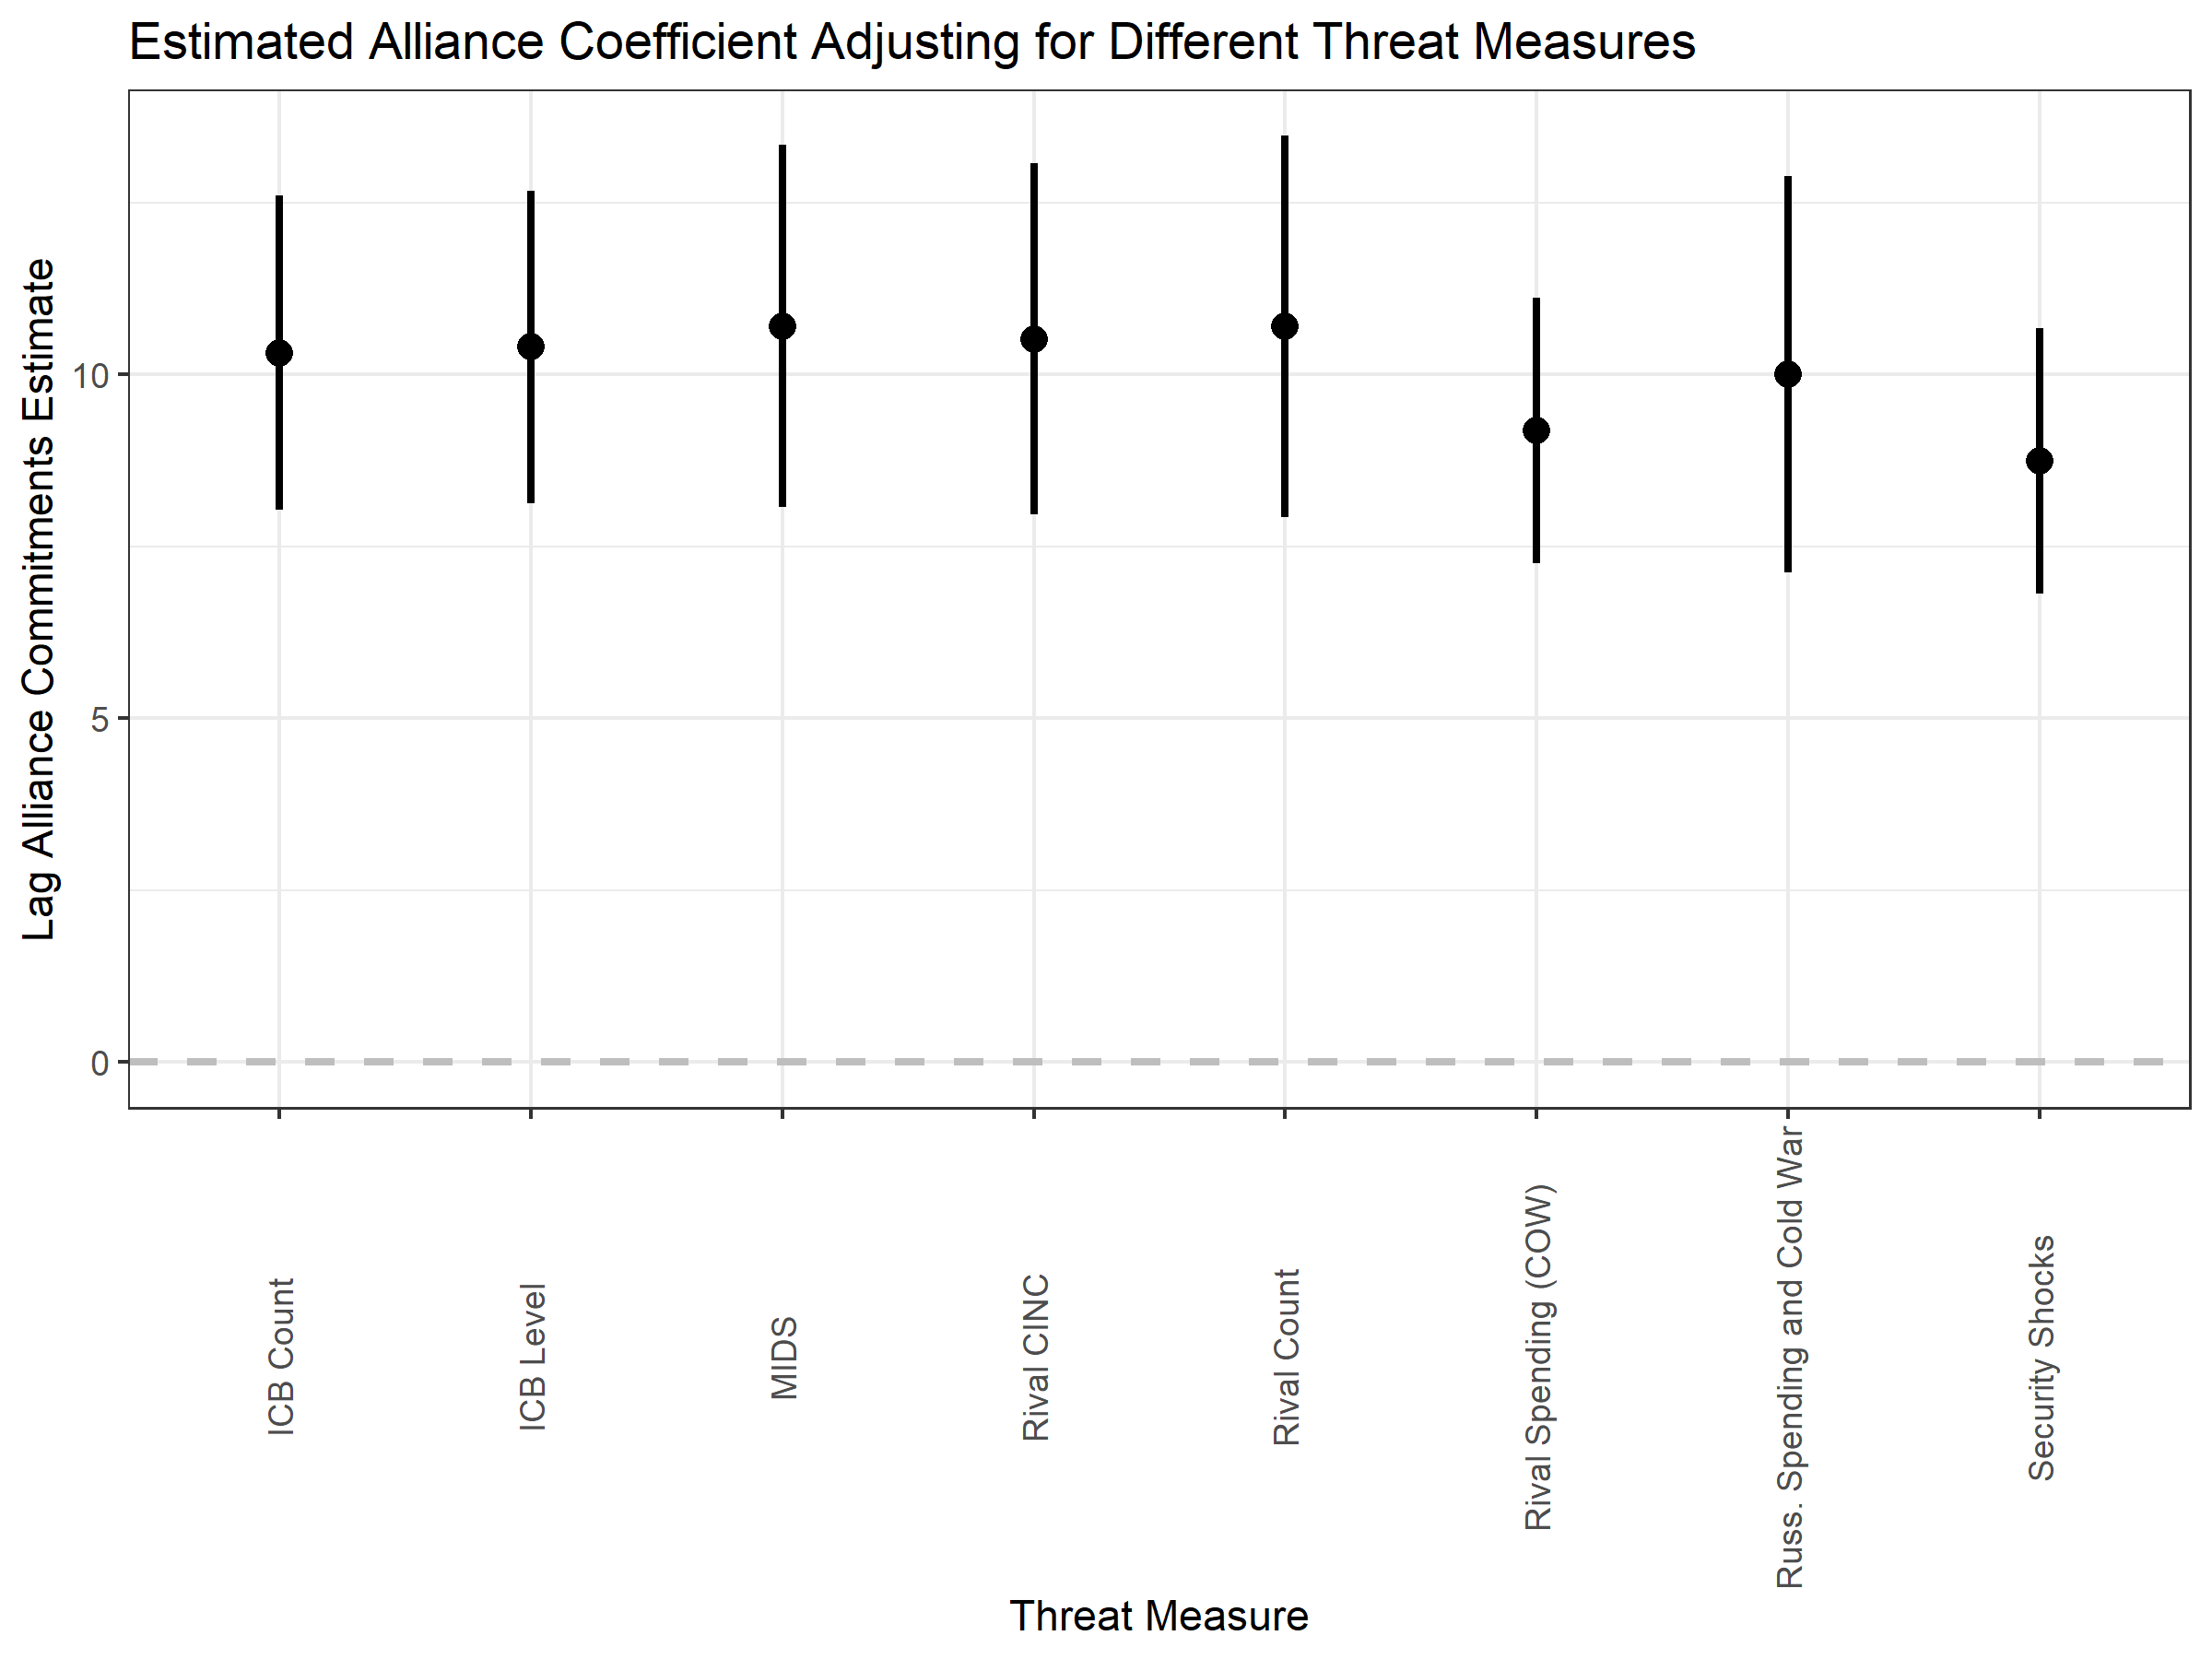
\includegraphics[width = .95\textwidth]{alt-threat-res.png}
\caption{Estimated association between U.S. alliance commitments and military spending across seven models with alternative controls for external threat.
Each point and range marks the coefficient estimate and 95\% confidence interval. 
Each estimate comes from a separate regression model, and models are labeled by their specific threat measure. }
\label{fig:alt-threat-res}
\end{figure}


\autoref{fig:alt-threat-res} plots the lag alliance commitments coefficient from seven OLS models with different threat indicators. 
In all of these models, our estimate of the association between alliance commitments and military spending is fairly consistent. 



\section{Counterfactual Plot of NATO Expansion with Logged Commitments} 

This section includes a figure summarizing the estimated impact of expanding NATO into the Baltic States, which we mention in the manuscript. 
\autoref{fig:nato-counterfactual-adl-log} shows the estimated impact of extending NATO to include Estonia, Latvia and Lithuania on U.S. military spending, based on estimates from observed data and predictions from counterfactual data without that part of NATO expansion.  


\begin{figure} 
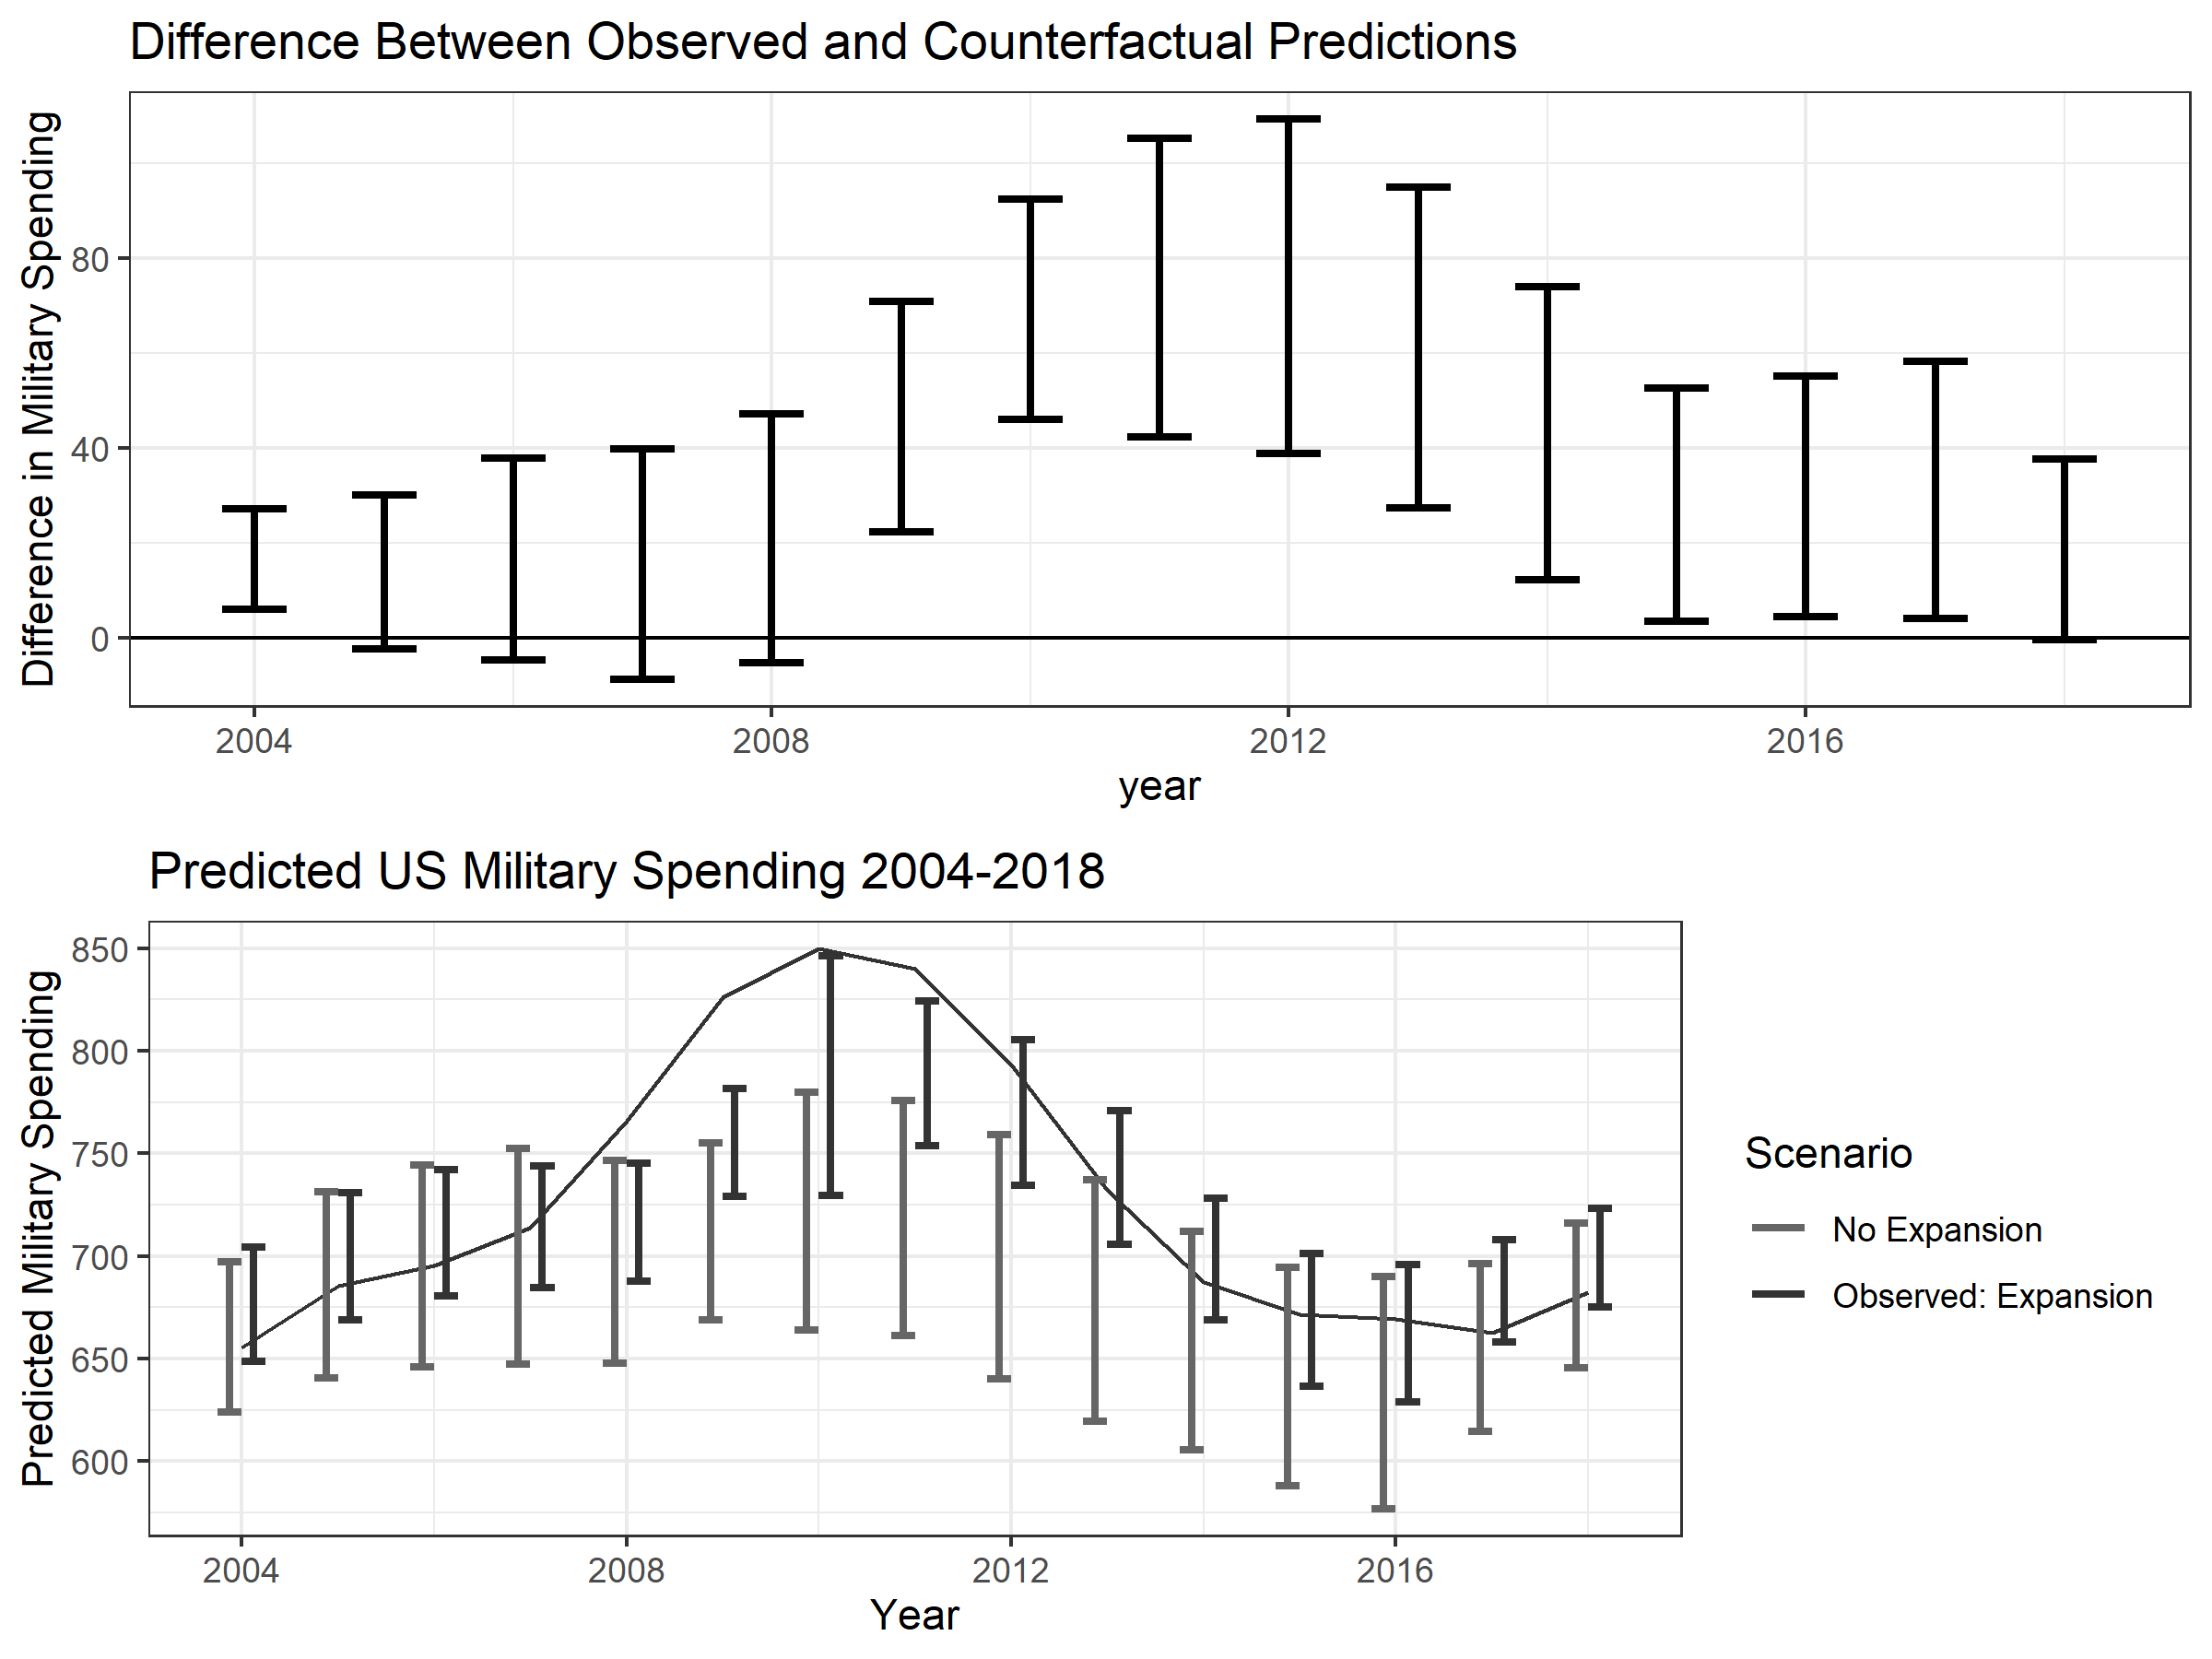
\includegraphics[width = .95\textwidth]{nato-counterfactual-adl-log.png}
\caption{Estimated U.S. military spending with and without NATO expansion to Estonia, Latvia and Lithuania. 
The bottom panel shows predictions from two circumstances: (1) observed NATO expansion and (2) a counterfactual scenario where NATO did not add the three Baltic countries in 2004. 
Estimates based on a model with logged alliance commitments. 
The top panel plots the estimated annual difference between predictions from the observed data. 
The error bars summarize the 95\% confidence interval for the predicted values and differences.
Estimates on the scale of billions of dollars.}
\label{fig:nato-counterfactual-adl-log}
\end{figure}




\section{Model Specification Uncertainty: Extreme Bounds Analysis} 


A possible critique of our findings in the paper is that the results are driven by a particular regression specification. 
Selecting control variables is difficult, and the choices we made could affect our inferences about alliance commitments. 
Put differently, perhaps alliance commitments are not a consistently strong predictor of military spending across different regression models. 


Standard robustness checks that add a few control variables at a time may not help this issue. 
The set of possible regression specifications far exceeds the number of models an analyst can reasonably specify manually.  
Therefore, we use extreme bounds analysis to asses the sensitivity of our alliance coefficient estimates to changes in regression model specification \citep{Sala-i-Martin1997}.
This analysis estimates a series of regression models with different combinations of control variables and assesses the distribution of regression coefficients across the full set of potential specifications.\footnote{For an example of an International Relations article that employs this analysis, see \citet{bellISQ16}.}
In this analysis, we focus on the distributions of the lagged alliance commitments coefficient.
The outcome is still annual military spending, and we include lagged spending levels in every specification. 

Our analysis spans 11,887 model specifications, which have different combinations of control variables in addition to lagged alliance commitments.  
We focus on the 1947-2019 sample for this analysis, and allow anywhere between zero and eight other variables in the model. 
The set of possible control variables include the variables in the main model of the manuscript, as well as the post-911 and pre-1952 dummies, the log of troops deployed in major combat operations, lagged levels of GDP, annual budget deficits, changes in GDP, and changes in the budget deficit. 


\begin{figure} 
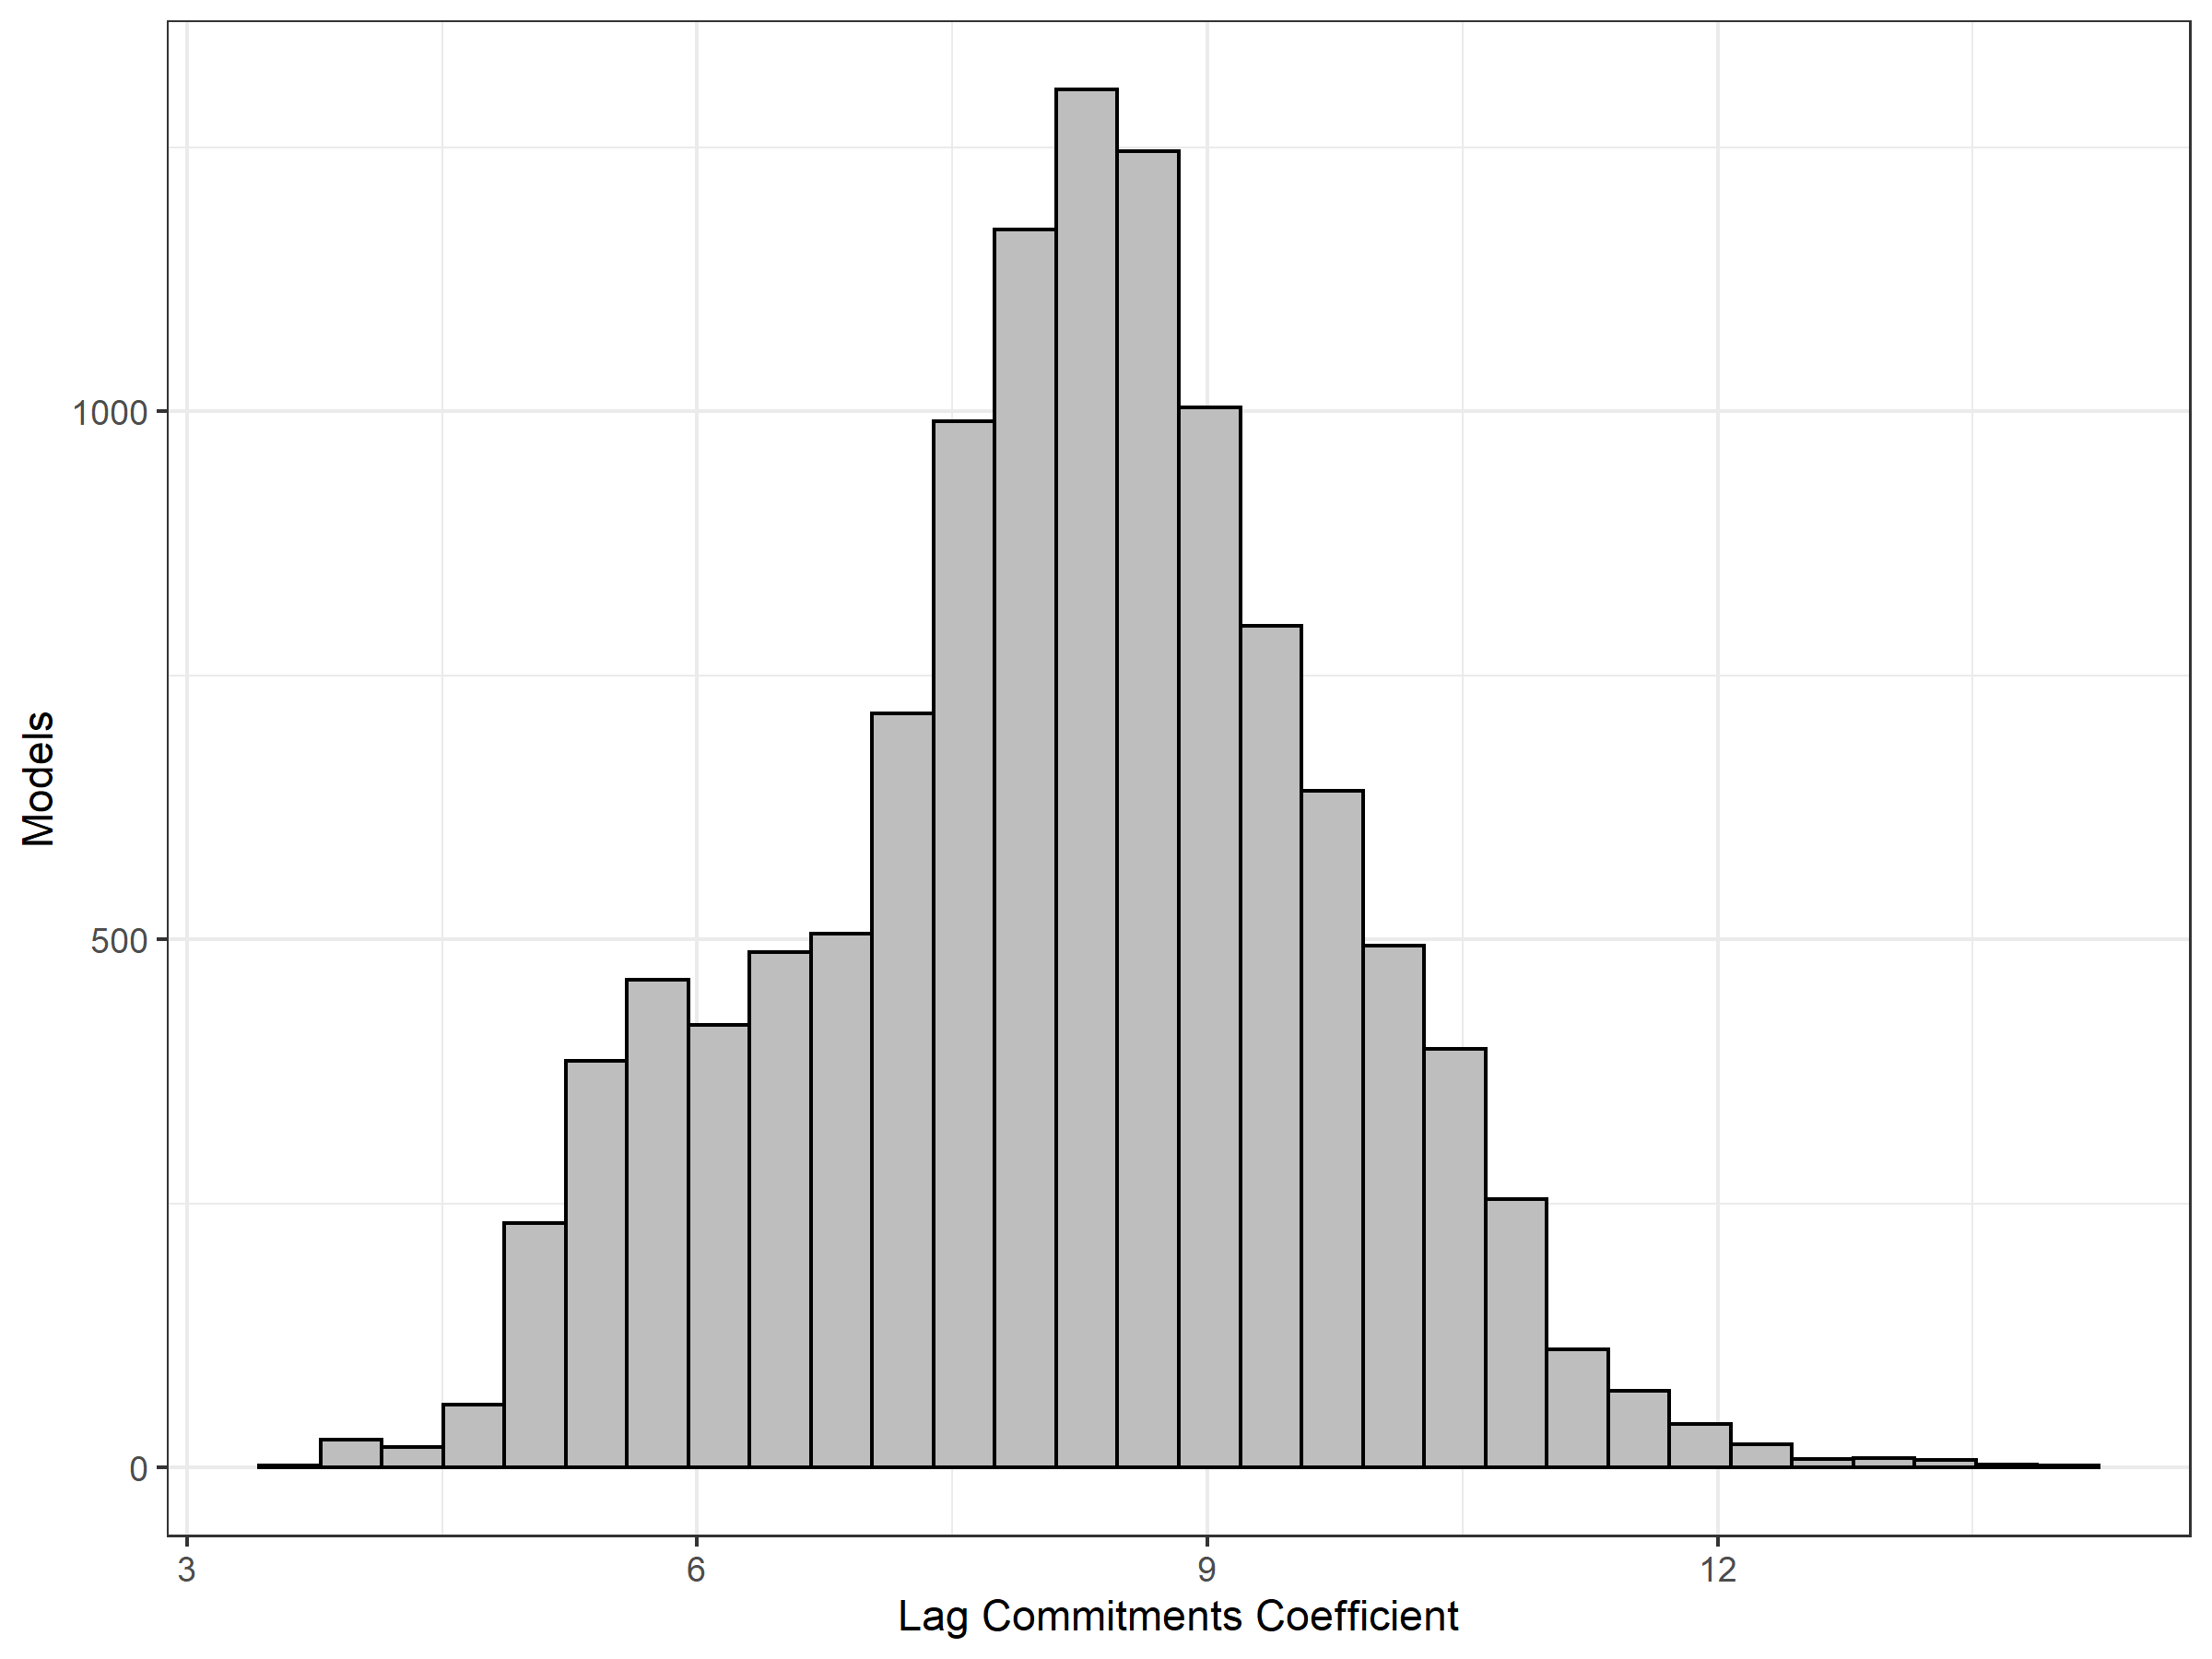
\includegraphics[width = .95\textwidth]{eba-res.png}
\caption{Histogram of the lagged alliance commitments regression coefficient across 12,911 possible regression model specifications.
The models contain different control variables, in addition to the alliance commitments and lagged spending variables.}
\label{fig:eba-res}
\end{figure}


We plot the distribution of the lagged alliance commitments coefficient across the 12,911 specifications in \autoref{fig:eba-res}. 
The lagged alliance commitments coefficient is positive across every model, and centered near the value of our coefficient estimate in the manuscript. 
There is variation in the coefficient estimate, but the bounds analysis may include models with residual autocorrelation or other regression assumption violations. 
While we took precautions to avoid biased or inefficient estimates in the models in the manuscript, these specifications may not have the same properties.  
Even so, our inferences about the likely coefficient on alliance commitments are relatively consistent across model specifications. 
No matter how the control variables in the model are set up, lagged alliance commitments are positively correlated with U.S. military spending. 


Substantive inferences about alliance commitments and military spending across thousands of regression models are also consistent with a large positive effect of alliances on U.S. military spending.
We plot the distribution of long-run multiplier estimates in \autoref{fig:lrm-eba}. 
The median estimate is \$14 billion, the minimum is \$6, and the maximum is 28. 
Ninety-five \% of these estimated long-run effects are between \$8 to \$20 billion.  


\begin{figure} 
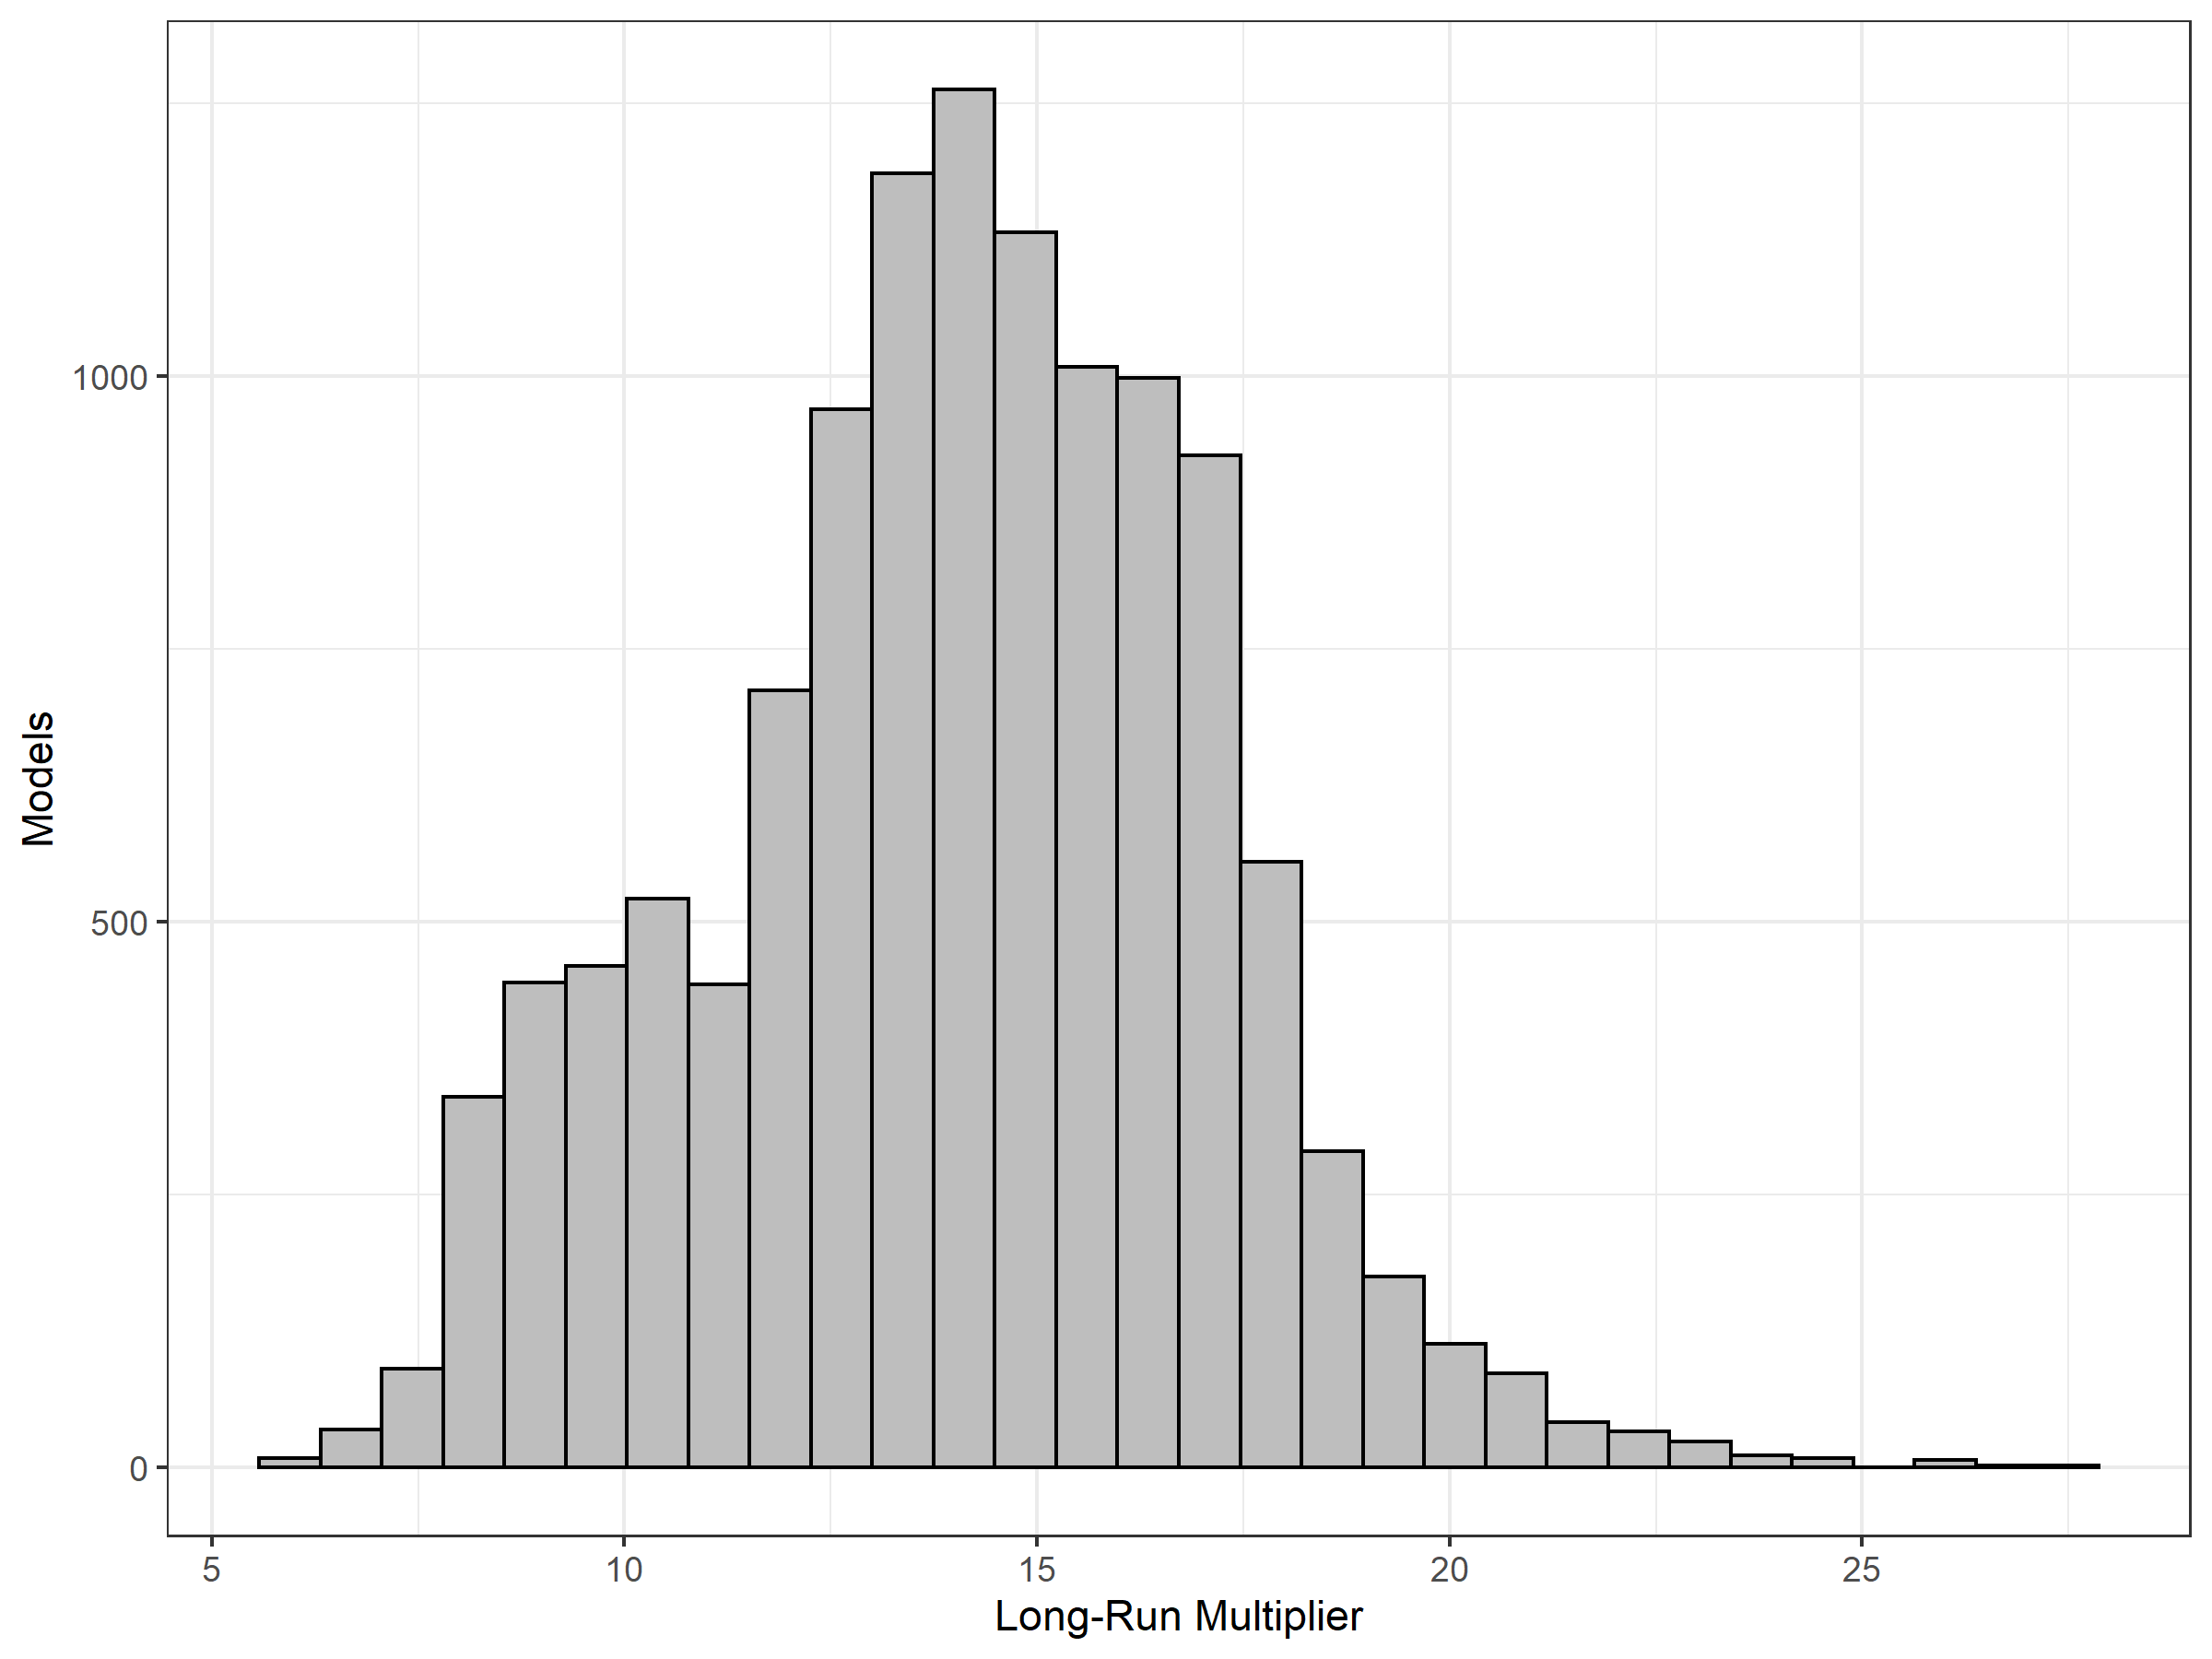
\includegraphics[width = .95\textwidth]{lrm-eba.png}
\caption{Histogram of estimated long-run impact of a one-unit increase in U.S. alliance commitments on military spending across 12,911 possible regression model specifications. 
The models contain different control variables, in addition to the alliance commitments and lagged spending variables.}
\label{fig:lrm-eba}
\end{figure}




\section{Sensitivity Analysis}


Confounding by unobserved factors is a further threat to our inferences in this paper. 
Although we adjust for a variety of observable variables, it is possible that some unobservable confounding factor is responsible for the strong positive correlation between alliance commitments and U.S. military spending. 
Theoretically, U.S. foreign policy interests and grand strategy in the post-war period and policymakers' expectations about the future are the most likely unobservables. 
We cannot rule the possibility of confounding by unobservables out entirely, but we can use our model to assess the implications of unobserved confounding using sensitivity analysis \citep{CinelliHazlett2020}. 


Sensitivity analysis uses model estimates to assess how large confounding by unobserved factors would have to be to reduce or eliminate an estimated relationship. 
Our analysis uses the main regression model from the manuscript. 
We then ask how severe confounding by unobservable factors would have to be to cut the lagged alliance commitments coefficient in half.
We chose this threshold because it creates a stringent test, and is roughly the threshold where the magnitude of the long-run relationship between alliances and spending might be consistent with the budget hawk view.
To facilitate substantive interpretation, our analysis benchmarks the strength of the hypothetical unobserved confounding factor to the log combat fatalities coefficient, as this war intensity measure is a strong predictor of military spending. 


This sensitivity analysis generates thresholds for three types of confounding. 
\autoref{tab:sensitivity-res} presents these results.
First, in an extreme case ($R^2_{Y \sim D |{\bf X}}$) where an unobserved confounder or some combination of several confounders explains 100\% of the residual variation in military spending, those factors would also have to explain 40\% of the variation in alliances to fully account for the association between alliance commitments and U.S. military spending.  
The next two numbers in \autoref{tab:sensitivity-res} express the percentage of the residual variation in alliance commitments and military spending that some unobservable factor would have to explain to reduce the alliance commitments coefficient estimate by half. 
$RV_{q = 0.5}$ shows that unobserved confounders that explain 33.8\% of such variation could cut the alliance commitments coefficient in half. 
$RV_{q = 0.5, \alpha = 0.05}$ expresses the same quantity, for a hypothesis test with a confidence level of .05.


\begin{table}[!h]
\centering
\begin{tabular}{lrrrrrr}
\multicolumn{7}{c}{Outcome: \textit{Military Spending}} \\
\hline \hline 
Treatment: & Est. & S.E. & t-value & $R^2_{Y \sim D |{\bf X}}$ & $RV_{q = 0.5}$ & $RV_{q = 0.5, \alpha = 0.05}$  \\ 
\hline 
\textit{Lag Alliance Commitments} & 9.67 & 1.466 & 3.297 & 40.8\% & 33.8\% & 14.9\% \\ 
\hline 
df = 63 & & \\%\multicolumn{5}{r}{ \small \textit{Bound (0.5x Log Combat Fatalities)}: $R^2_{Y\sim Z| {\bf X}, D}$ = 16\%, $R^2_{D\sim Z| {\bf X} }$ = 0.2\%} \\
\end{tabular}
\caption{Results from sensitivity analysis of the association between lagged alliance commitments and U.S. military spending, 1947 to 2020.}
\label{tab:sensitivity-res}
\end{table}


These estimates suggest that substantial unobserved confounding is necessary to even reduce the estimated association between alliances and spending by 50\%. 
This sensitivity analysis cannot rule out unobserved confounding, but it establishes the necessary magnitude of any confounding. 
Seeing as our models account for many salient observables, we suspect that remaining unobservables are probably not strong enough predictors of alliances and spending to change our substantive inferences.



\section{Error Correction Models} 


Error correction models are an alternative way to specify dynamic regression models.\footnote{The general error correction model is algebraically equivalent to a autoregressive dynamic lag model \citep{DeBoefKeele2008}.}
Though we do not use this model for the results in the manuscript, it produces very similar inferences about the substantive impact of alliance commitments on U.S. military spending. 
An error correction model employs linear regression to estimate a long-run equilibrium relationship through levels and changes of key variables.
Our general error correction model includes both the previous year's number of alliance commitments and the change in alliance commitments in each year as the key independent variables. 
The dependent variable is annual changes in the U.S. defense budget.
We then include the lagged level of the previous year's defense budget and the previous annual change in military spending on the right-hand side of the equation.
These lagged values imply that present military spending decisions depend on past increases or decreases in the defense budget as well as the level of defense spending.


An error correction specification is only appropriate if two conditions are met, however. 
First, we need to know whether there is a long-run relationship between alliances and defense spending. 
Second, we must establish that alliances and defense spending are cointegrated. 
Although there is ample debate about using error correction models in other situations, scholars agree that error correction is appropriate for cointegrated variables\citep{EngleGranger1987, DeBoefKeele2008, GrantLebo2016, Ennsetal2016}. 
Cointegration means that the a linear combination of non-stationary variables is stationary, which implies a long-run equilibrium.  
We carried out tests to assess if these two conditions are satisfied. 
First, we applied the same long-run multiplier bounds test reported in the manuscript,\footnote{In an error correction model, the estimated long-run effect of alliances is equal to $-\frac{\mbox{Lag Alliance Commitments}}{Lag Military Spending}$.} and the estimates suggest that a long-run relationship is present. 


% cointegration tests
After establishing that there is likely a long-run relationship between alliances and defense spending, we tested for cointegration. 
If alliances and military spending are cointegrated, an equilibrium relationship is likely present, and an error correction model is appropriate.    
Consistent with best practices, we applied a battery of tests and found evidence of cointegration \citep{Philips2018}. 
We first ensured that all variables are stationary or first order integrated. 
Then we estimated an error correction model and added lags of the dependent and independent variables until the residuals were white noise. 
Finally, we applied the bounds cointegration test to examine the model for cointegration. With this test, we reject the null of no cointegration at the 1\% level with both t and F-tests. 
We also repeated the procedure using a model with linear trend and made similar inferences. 
The coefficient estimates with a linear trend term are also very similar.


Given evidence of cointegration, why do we use an autoregressive distributed lag (ADL) model in the paper instead of an error correction model? 
There are two reasons we highlight the ADL model results. 
First, interpreting the ADL estimates is slightly more straightforward. 
Second, and more importantly, the cointegration tests assume that the outcome --- military spending in our analysis --- is a unit root. 
Unfortunately, given the limits of unit root tests like the Dickey-Fuller test in small samples, we cannot say for sure whether U.S. military spending is a unit root. 
A battery of unit root tests gives conflicting answers about the time-series properties of US military spending. 
Moreover, unit root tests are not particularly powerful in small samples. 
If military spending is a unit root, the long-run multiplier bounds test should still give reasonable substantive estimates, and it applies to both ADL and error correction models.


Model specification debates aside, our substantive inferences about alliances and U.S. military spending are very similar in the error correction model specification.
We estimate the same mix of models as the manuscript--- one error correction model uses the number of the commitments as the key independent variable and another employs logged commitments. 
\autoref{tab:ecm-coefs} presents the coefficient estimates from these two models. 


\begin{table}[!htbp] \centering  
\begin{adjustbox}{width= .95\textwidth, center}
\begin{tabular}{@{\extracolsep{5pt}}lcc} 
\\[-1.8ex]\hline \\[-1.8ex] 
\\[-1.8ex] & \multicolumn{2}{c}{Change in Military Spending} \\ 
\\[-1.8ex] & (1) & (2)\\ 
\hline \\[-1.8ex] 
 Lagged Military Spending & $-$0.466$^{}$ & $-$0.426$^{}$ \\ 
  & ($-$0.605, $-$0.328) & ($-$0.564, $-$0.287) \\ 
  Lag Changes in Military Spending & 0.248$^{}$ & 0.260$^{}$ \\ 
  & (0.109, 0.387) & (0.080, 0.439) \\ 
  Lag Alliance Commitments & 5.405$^{}$ &  \\ 
  & (1.560, 9.250) &  \\ 
  Change Alliance Commitments & 4.366 &  \\ 
  & ($-$1.517, 10.249) &  \\ 
  Lag Log Alliance Commitments &  & 138.803$^{}$ \\ 
  &  & ($-$19.228, 296.835) \\ 
  Change in Log Alliances &  & 166.621 \\ 
  &  & ($-$64.583, 397.826) \\ 
  Lag Change in GDP & $-$0.025 & $-$0.005 \\ 
  & ($-$0.090, 0.039) & ($-$0.069, 0.059) \\ 
  Cold War & $-$10.951 & $-$49.684 \\ 
  & ($-$84.269, 62.366) & ($-$117.025, 17.657) \\ 
  Lag Rival Spending & 0.051 & 0.084$^{}$ \\ 
  & ($-$0.041, 0.142) & ($-$0.007, 0.174) \\ 
  Post-Conflict Years & $-$6.057 & $-$10.075 \\ 
  & ($-$29.568, 17.455) & ($-$34.225, 14.074) \\ 
  Log Combat Fatalities & 6.295$^{}$ & 6.411$^{}$ \\ 
  & (2.630, 9.960) & (2.498, 10.325) \\ 
  Lag Republican President & 16.911 & 20.279$^{}$ \\ 
  & ($-$4.114, 37.936) & ($-$1.377, 41.935) \\ 
  Lag Budget Deficit & $-$1.709 & $-$2.585 \\ 
  & ($-$7.812, 4.393) & ($-$8.849, 3.680) \\ 
  Constant & $-$55.148 & $-$339.381 \\ 
  & ($-$237.663, 127.366) & ($-$940.921, 262.158) \\ 
 N & 73 & 73 \\ 
\hline \\[-1.8ex] 
\multicolumn{3}{l}{95\% Confidence Intervals in Parentheses.} \\ 
\end{tabular} 
\end{adjustbox}
  \caption{Error correction models of alliances and U.S. military spending from 1947 to 2019. 
  Model 1 uses the number of alliance commitments, while Model 2 uses logged alliance commitments.} 
  \label{tab:ecm-coefs}
\end{table} 


The change in alliance commitments coefficient captures the immediate effect of adding new security guarantees.
Based on Model 1, adding one additional commitment increases U.S. defense spending by \$4 billion.
The 95 percent confidence interval indicates that the immediate effect could range between \$-2 and \$10 billion.
Thus, adding one commitment to the U.S. alliance portfolio probably has a positive impact on short-run expenditures, but the estimate is also consistent with a small negative or no effect. 
The same unclear short-run impact is present in logs as well. 
This makes sense because we would not expect new alliances to affect the defense budget in the same year they are formed.

On the other, the lagged alliance commitment is large and positive in both commitment levels and logged commitments. 
In this model, the lagged alliance commitment coefficient does not express the total impact of a change in alliances. 
To calculate the substantive impact of changes in alliance commitments, we again rely on the long-run multiplier bounds test. 
In an error correction model, the long-run multiplier is equal to $-\frac{\mbox{Lag Commitments}}{\mbox{Lagged Spending}}$, and the standard errors can still be calculated with the Delta method. 
In expectation, the alliance long-run multiplier in the error correction model suggests that one new alliance commitment increases US military spending by \$12 billion. 
The 95\% interval of this estimate ranges between 4 and 19 billion, so the key substantive inference is very similar to the ADL model in the manuscript, albeit with slightly greater uncertainty. 
Independent variables have a less intuitive interpretation when they are log-transformed, but Model 2 similarly yields a potentially large substantive effect.  
A 10 percent increase in the logged alliance commitments leads to about \$43 billion more in defense spending, with a 95 percent confidence interval ranging from \$76 billion to \$10 billion.
Therefore, an error correction model gives very similar substantive inferences about the connection between alliances and military spending. 



\section{Changes in Spending and Changes in Commitments} 


Modeling the dynamic relationship between alliances and defense spending is at the core of our analysis. 
We make similar inferences about alliance commitments and U.S. military spending with a more static model, however. 
The static model removes the lagged levels of alliance participation and military spending that are essential to the error correction model, and replaces them with lagged changes in alliances and changes in spending. 


Modeling changes in spending as a function of changes in alliances reflects a very different theoretical argument.
These models assume that the effect of a change in alliance obligations dissipates fairly rapidly. 
Neither the bargain hunter nor the budget hawk perspective claims that the effect of changes in alliances will be realized quite in such a short time span.   
Even so, results with more static models are largely consistent with our findings in the paper. 


To ensure these models do not violate crucial regression assumptions, we control for lagged spending changes. 
Adding this variable reduces residual autocorrelation. 
It also means that even after expressing the relationship in first differences, some remnants of military spending dynamics remain. 


To account for unusual observations, we complement ordinary least square estimation with robust regression. 
Robust regression places less weight on unusual observations that have large regression residuals.
As such, robust regression estimates are less sensitive to large increases or decreases in military spending. 
As a further check on the influence of unusual spending changes, we add decade and presidential fixed effects in some models. 


\begin{figure} 
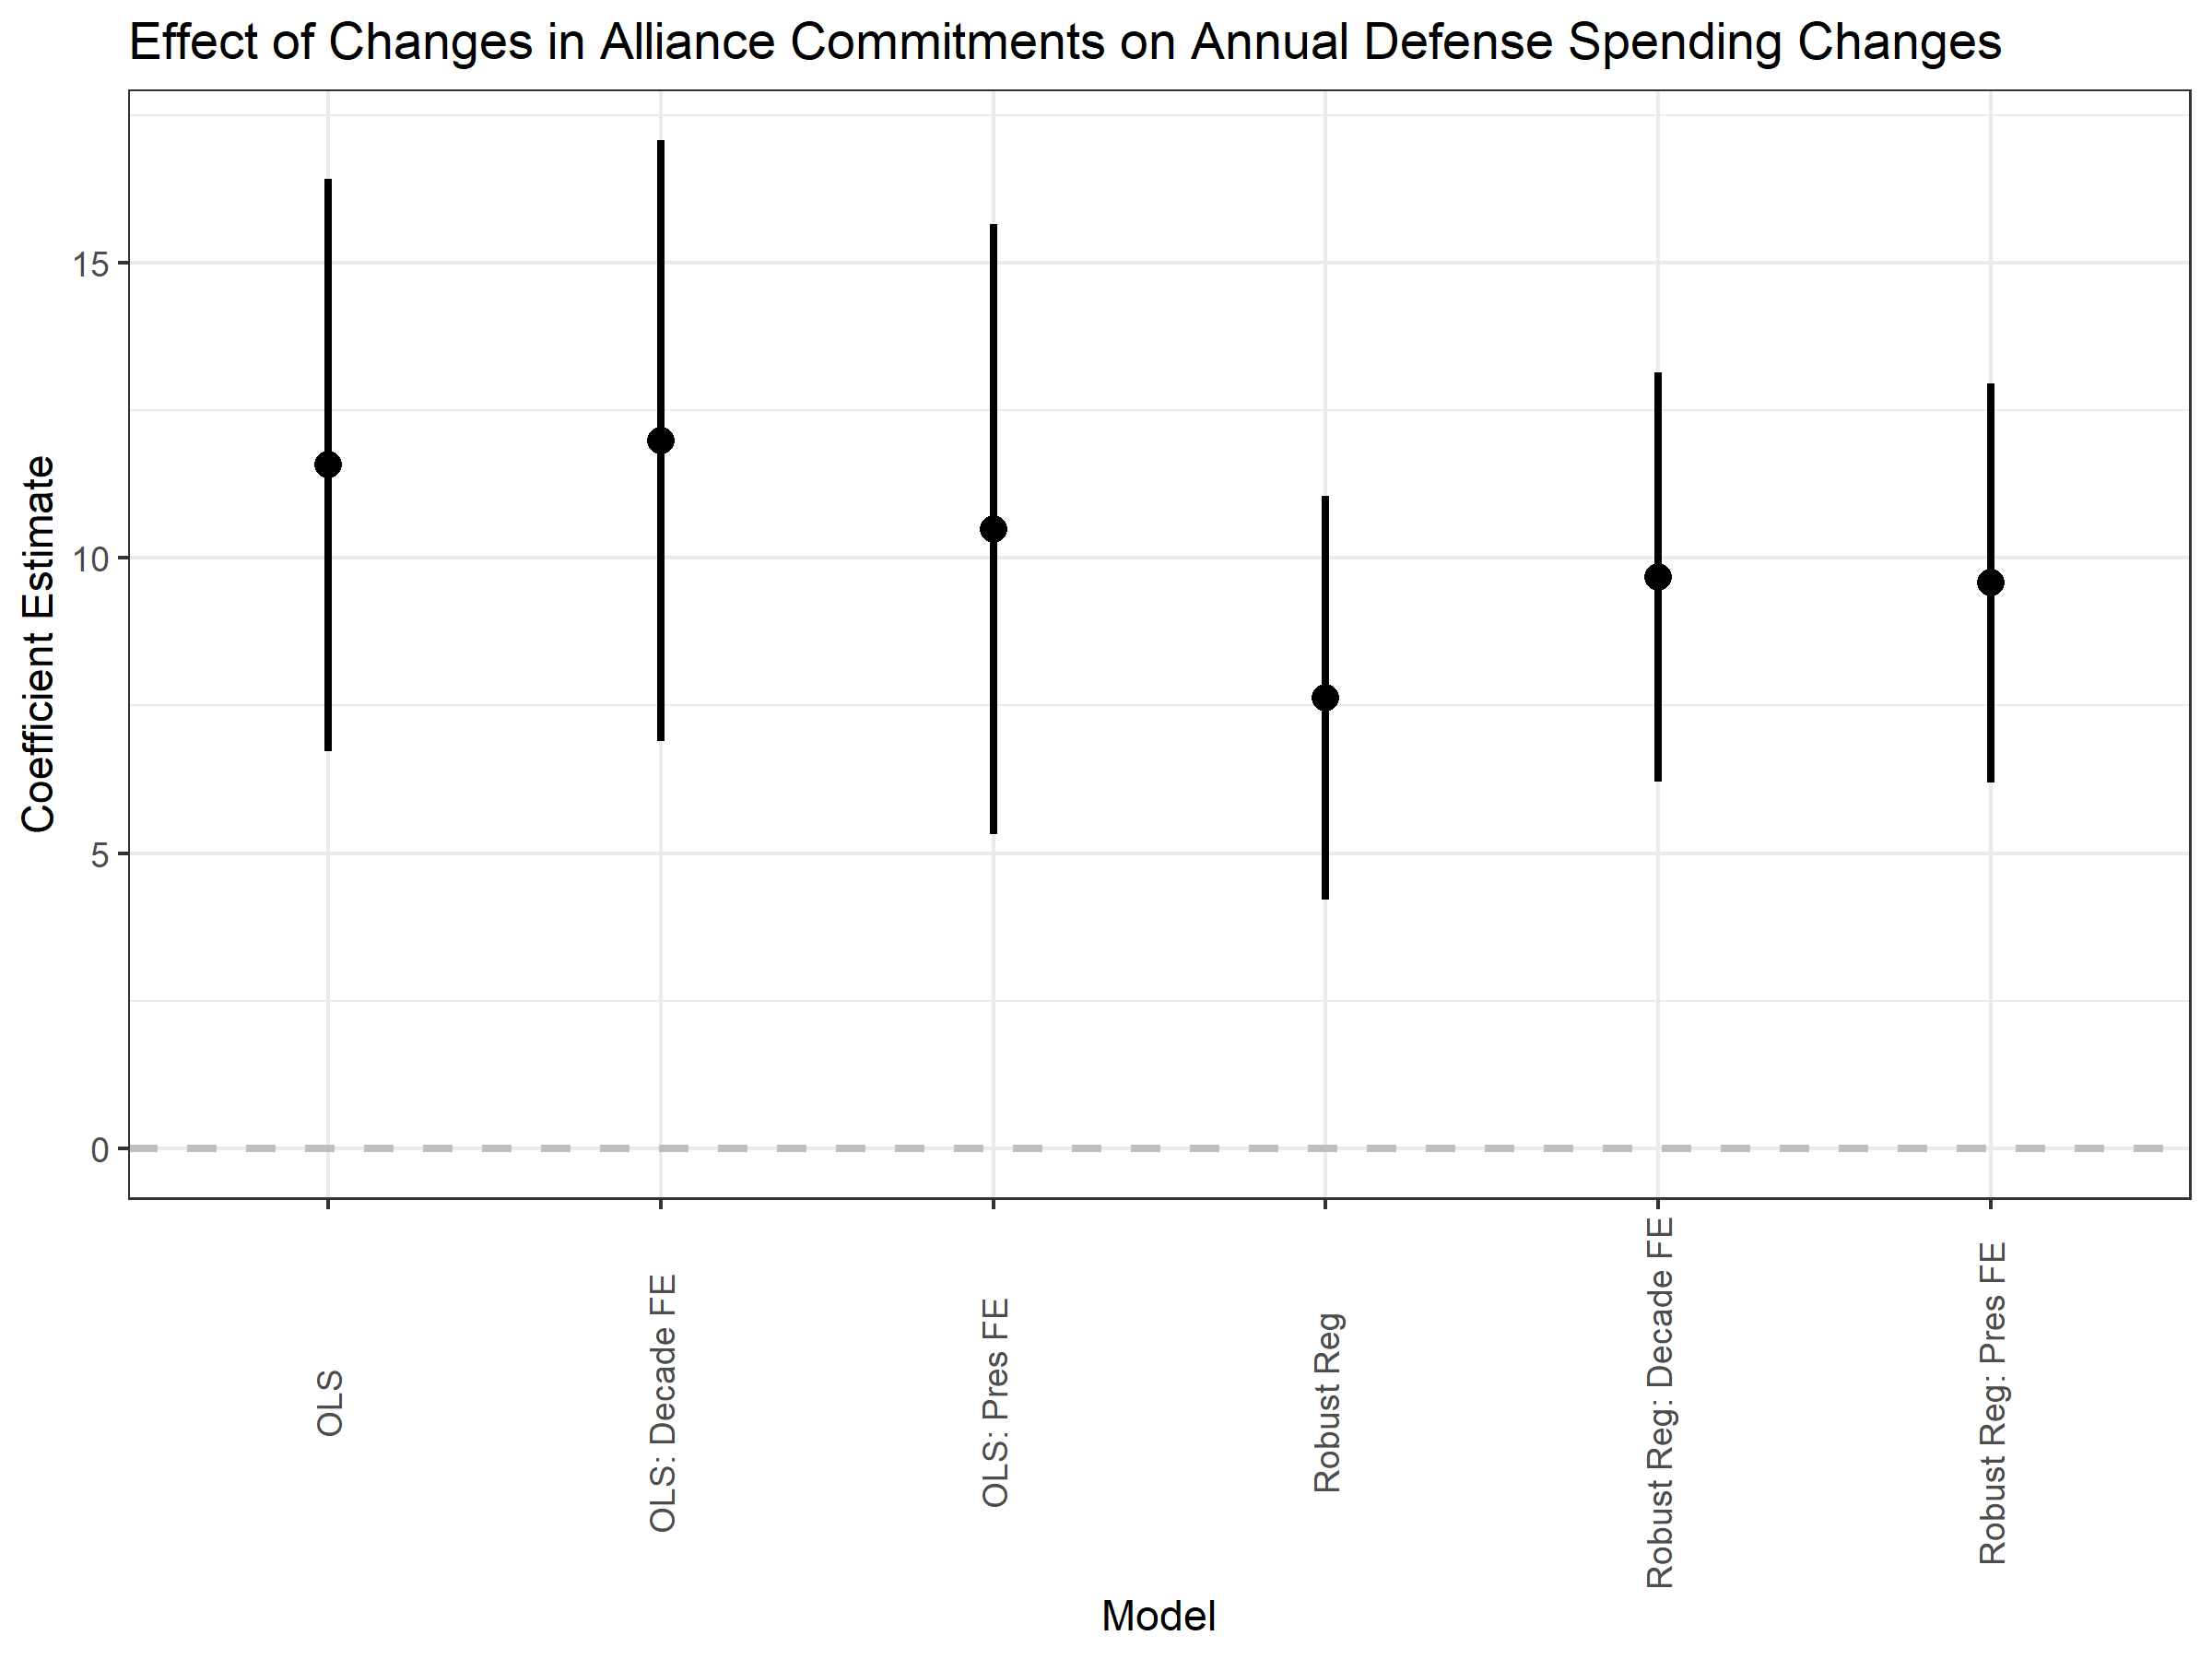
\includegraphics[width = .95\textwidth]{change-coefplot.png}
\caption{Effect of lagged changes in alliance commitments on annual changes in U.S. military spending from 1947 to 2019.
These coefficients reflect the initial impact of a new alliance commitment.}
\label{fig:change-coefplot}
\end{figure}


We present the estimated effect of changes in alliance commitments on changes in military spending across six different models of spending changes and alliance changes in \autoref{fig:change-coefplot}. 
All six estimates are clearly positive and have a large magnitude. 
These estimates imply that increasing alliance commitments adds to annual changes in the U.S. defense budget. 
Results are robust to decade and presidential fixed effects. 


Because we control for lagged spending changes, we can still calculate the total effect of an increase in alliance commitments. 
\autoref{fig:changes-long-run-est} presents these results, which are based on the lagged changes and lagged change in alliance commitments coefficients.
The substantive effect of a change in alliances is roughly equivalent to our findings in the manuscript. 
In expectation, one new alliance commitment adds roughly \$15 billion to annual changes in U.S. military spending. 


\begin{figure} 
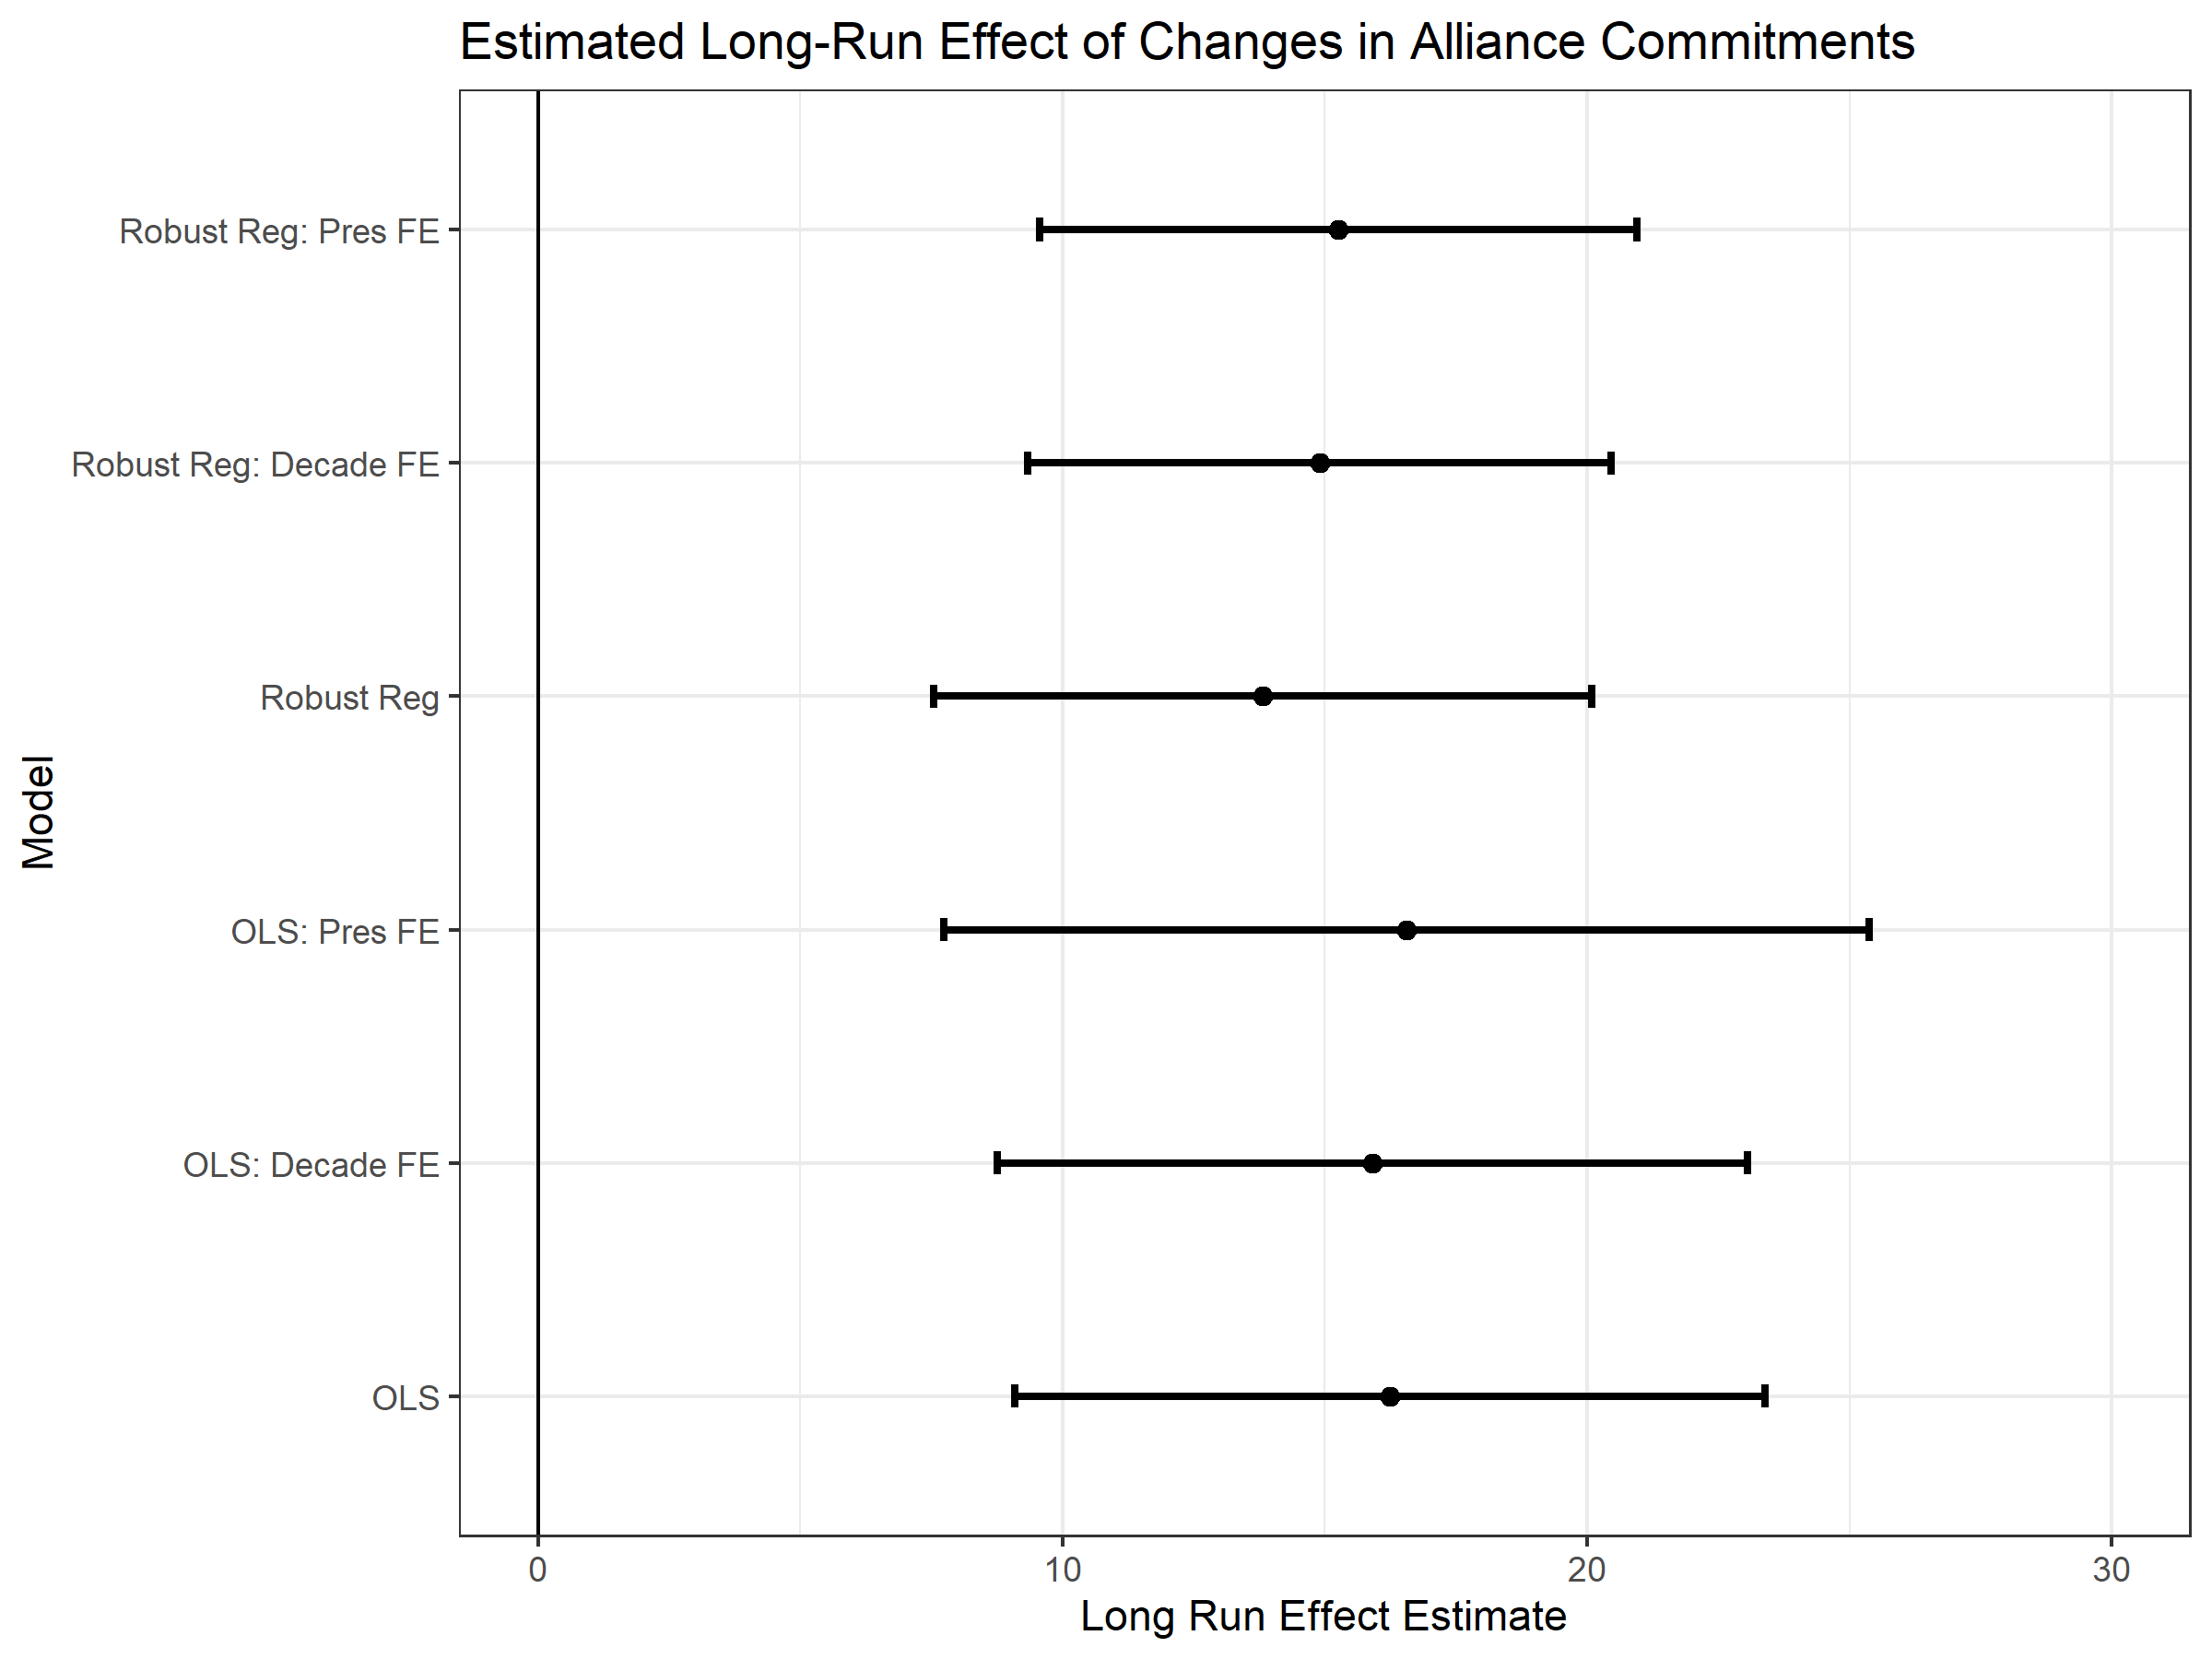
\includegraphics[width = .95\textwidth]{changes-long-run-est.png}
\caption{Total effect of a one-unit increase in lagged changes in alliance commitments on annual changes in U.S. military spending from 1947 to 2019.
These estimates capture the full impact of a new alliance commitment on annual spending changes.}
\label{fig:changes-long-run-est}
\end{figure}



\section{Analysis from 1920 to 2012}


Our model in the manuscript analyzes military spending and alliances from 1947 to 2019. 
As a result, the number of alliance commitments has a minimum value of 20. 
This leaves substantial variation in alliance commitments, but alliance commitments are never at 0 thanks to carryover of Western Hemisphere alliances from World War II to the Cold War period. 
In this section, we extend the military spending data back to 1920 and analyze the relationship between alliances and military spending from 1920 to 2012.
This analysis ends in 2012 because we use a measure of rival capability based on the CINC data \citep{SingerCINC1988}, and the most recent CINC data ends in 2012.


We do not report these results in the manuscript for two reasons.
First, our military spending measure is an amalgamation of data from multiple sources, and we rebase these measures to have a common base in 2018 U.S. dollars. 
This raises the prospect of measurement error. 
We also are missing several crucial controls due to missing data before 1945, though we include dummy indicators of World War II and years after 1945 to capture structural shifts.
We also adjust for the total CINC scores of U.S. strategic rivals. 
Regression modeling is also complicated by the massive changes in military spending during World War II shown in \autoref{fig:pre45-outcome-iv}, which generates huge outliers. 
Log-transforming military spending to pull in the WW2 outliers changes defense spending dynamics.  



\begin{figure} 
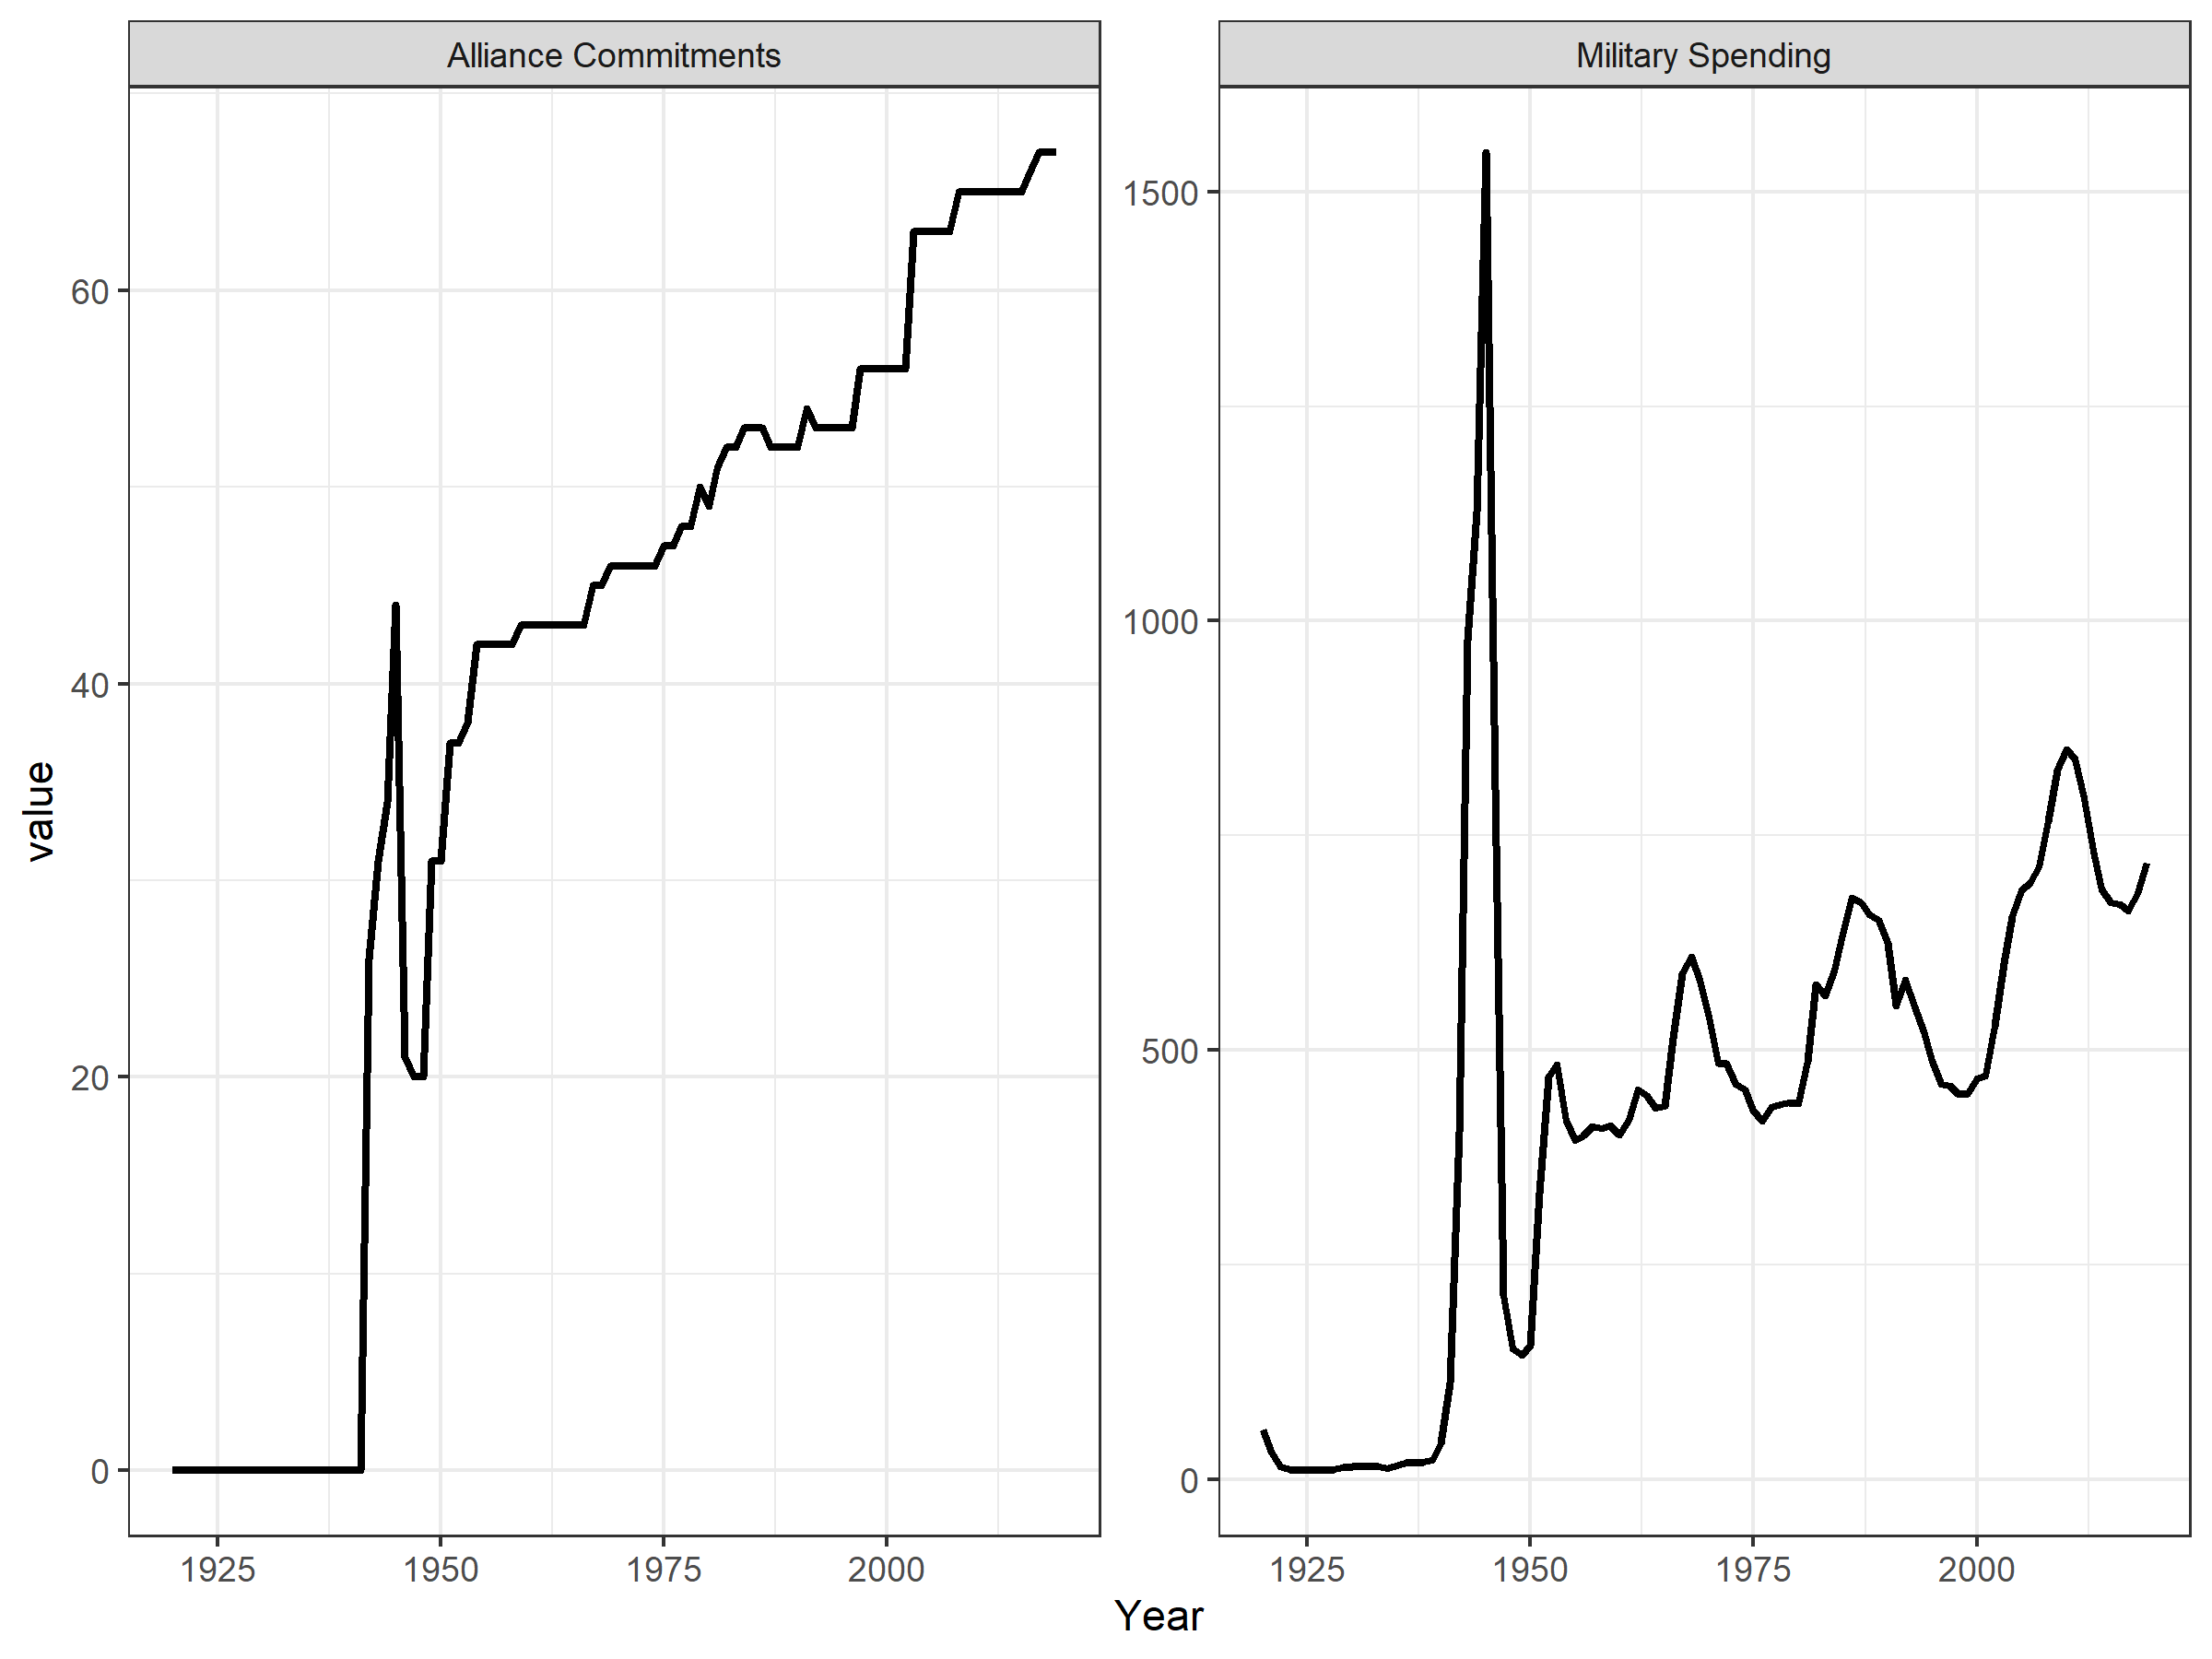
\includegraphics[width = .95\textwidth]{pre45-outcome-iv.png}
\caption{U.S. alliance commitments and military spending from 1920 to 2019.}
\label{fig:pre45-outcome-iv}
\end{figure}


Although the above issues mean that these results should be treated with caution, the results are similar when we extend the period of analysis from 1920 to 2012. 
This includes standard linear regression, robust regression, and the same estimators with logged alliances or presidential fixed effects.
In all these specifications, we estimate a positive relationship between alliance commitments and military spending. 
In the baseline linear regression, there is clear evidence of a long-run relationship between alliances and military spending with the long-run multiplier bounds test statistics of ten \citet{Webbetal2019}. 


We summarize association between alliance commitments and U.S. military spending from 1920 to 2012 in \autoref{tab:adl-coefs-pre45} and \autoref{fig:lrm-rob-pre45}. 
\autoref{tab:adl-coefs-pre45} shows the regression coefficients and confidence intervals. 
\autoref{fig:lrm-rob-pre45} then plots the estimated long-run multiplier of a change in alliance commitments for each model.
In the logged alliance commitments models, the long-run multiplier expresses the impact of a 10\% increase in alliances, which is the same change we report in the manuscript. 


\begin{sidewaystable}[!htbp] \centering  
\begin{adjustbox}{width= \textwidth}
\begin{tabular}{@{\extracolsep{5pt}}lcccccc} 
\\[-1.8ex]\hline \\[-1.8ex] 
\\[-1.8ex] & \multicolumn{6}{c}{Military Spending} \\ 
\\[-1.8ex] & (1) & (2) & (3) & (4) & (5) & (6)\\ 
\hline \\[-1.8ex] 
 Lagged Military Spending & 0.496$^{}$ & 0.471$^{}$ & 0.610$^{}$ & 0.598$^{}$ & 0.663$^{}$ & 0.643$^{}$ \\ 
  & (0.401, 0.591) & (0.387, 0.555) & (0.428, 0.791) & (0.549, 0.648) & (0.609, 0.718) & (0.591, 0.696) \\ 
  Lag Alliance Commitments & 9.944$^{}$ &  & 14.671$^{}$ & 6.857$^{}$ &  & 14.426$^{}$ \\ 
  & (7.616, 12.272) &  & (7.621, 21.720) & (5.644, 8.070) &  & (12.401, 16.450) \\ 
  Lag Log Alliance Commitments &  & 197.840$^{}$ &  &  & 183.899$^{}$ &  \\ 
  &  & (161.086, 234.593) &  &  & (159.854, 207.943) &  \\ 
  Post-Conflict Years & $-$24.011 & $-$55.658$^{}$ & $-$18.289 & $-$22.372$^{}$ & $-$28.748$^{}$ & 15.256 \\ 
  & ($-$61.755, 13.734) & ($-$87.816, $-$23.501) & ($-$94.373, 57.794) & ($-$42.037, $-$2.706) & ($-$49.786, $-$7.710) & ($-$6.593, 37.104) \\ 
  Total Rival CINC & 287.238$^{}$ & 129.045 & 611.252$^{}$ & 154.005$^{}$ & 115.131$^{}$ & 174.442$^{}$ \\ 
  & (67.910, 506.567) & ($-$63.153, 321.242) & ($-$91.080, 1,313.585) & (39.731, 268.279) & ($-$10.608, 240.870) & ($-$27.245, 376.129) \\ 
  World War II & 348.806$^{}$ & 155.501$^{}$ &  & 338.036$^{}$ & 95.065$^{}$ &  \\ 
  & (257.033, 440.580) & (62.126, 248.877) &  & (290.220, 385.851) & (33.977, 156.153) &  \\ 
  Post 1945 & $-$253.382$^{}$ & $-$513.968$^{}$ &  & $-$141.494$^{}$ & $-$551.716$^{}$ &  \\ 
  & ($-$359.151, $-$147.613) & ($-$641.914, $-$386.022) &  & ($-$196.601, $-$86.386) & ($-$635.420, $-$468.011) &  \\ 
  Lag Republican President & 13.027 & 32.341$^{}$ &  & 13.601 & 14.881 &  \\ 
  & ($-$19.118, 45.172) & (4.719, 59.963) &  & ($-$3.147, 30.349) & ($-$3.190, 32.952) &  \\ 
  Lag GDP Change & $-$0.00000 & 0.00000 & 0.00000 & $-$0.00000 & 0.00000 & 0.00000 \\ 
  & ($-$0.00000, 0.00000) & ($-$0.00000, 0.00000) & ($-$0.00000, 0.00000) & ($-$0.00000, 0.00000) & ($-$0.00000, 0.00000) & ($-$0.00000, 0.00000) \\  
  Constant & $-$23.836 & $-$16.564 & $-$759.919$^{}$ & $-$12.933 & $-$10.707 & $-$665.904$^{}$ \\ 
  & ($-$70.708, 23.036) & ($-$58.183, 25.055) & ($-$1,165.565, $-$354.272) & ($-$37.355, 11.488) & ($-$37.935, 16.521) & ($-$782.392, $-$549.416) \\ 
 N & 90 & 90 & 90 & 90 & 90 & 90 \\ 
\hline \\[-1.8ex] 
\multicolumn{7}{l}{95\% Confidence Intervals in Parentheses. Models 1-3 estimated with OLS.
          Models 4-6 estimated with robust regression. Presidential fixed effects omitted.} \\ 
\end{tabular} 
\end{adjustbox}
  \caption{OLS and robust regression estimates of the relationship between alliance commitments and U.S. military spending, 1920 to 2012. Models 1-3 estimated with OLS. Models 4-6 estimated with robust regression. Presidential fixed effects omitted from Models 3 and 6.} 
  \label{tab:adl-coefs-pre45} 
\end{sidewaystable} 


As \autoref{fig:lrm-rob-pre45} shows, the long run multiplier estimates for alliances in logs and with presidential fixed effects are extremely large.
These estimates, though they are consistent with our other findings, are likely inflated by World War II and the unusual dynamics of alliances and military spending between 1920 and 2012. 


\begin{figure} 
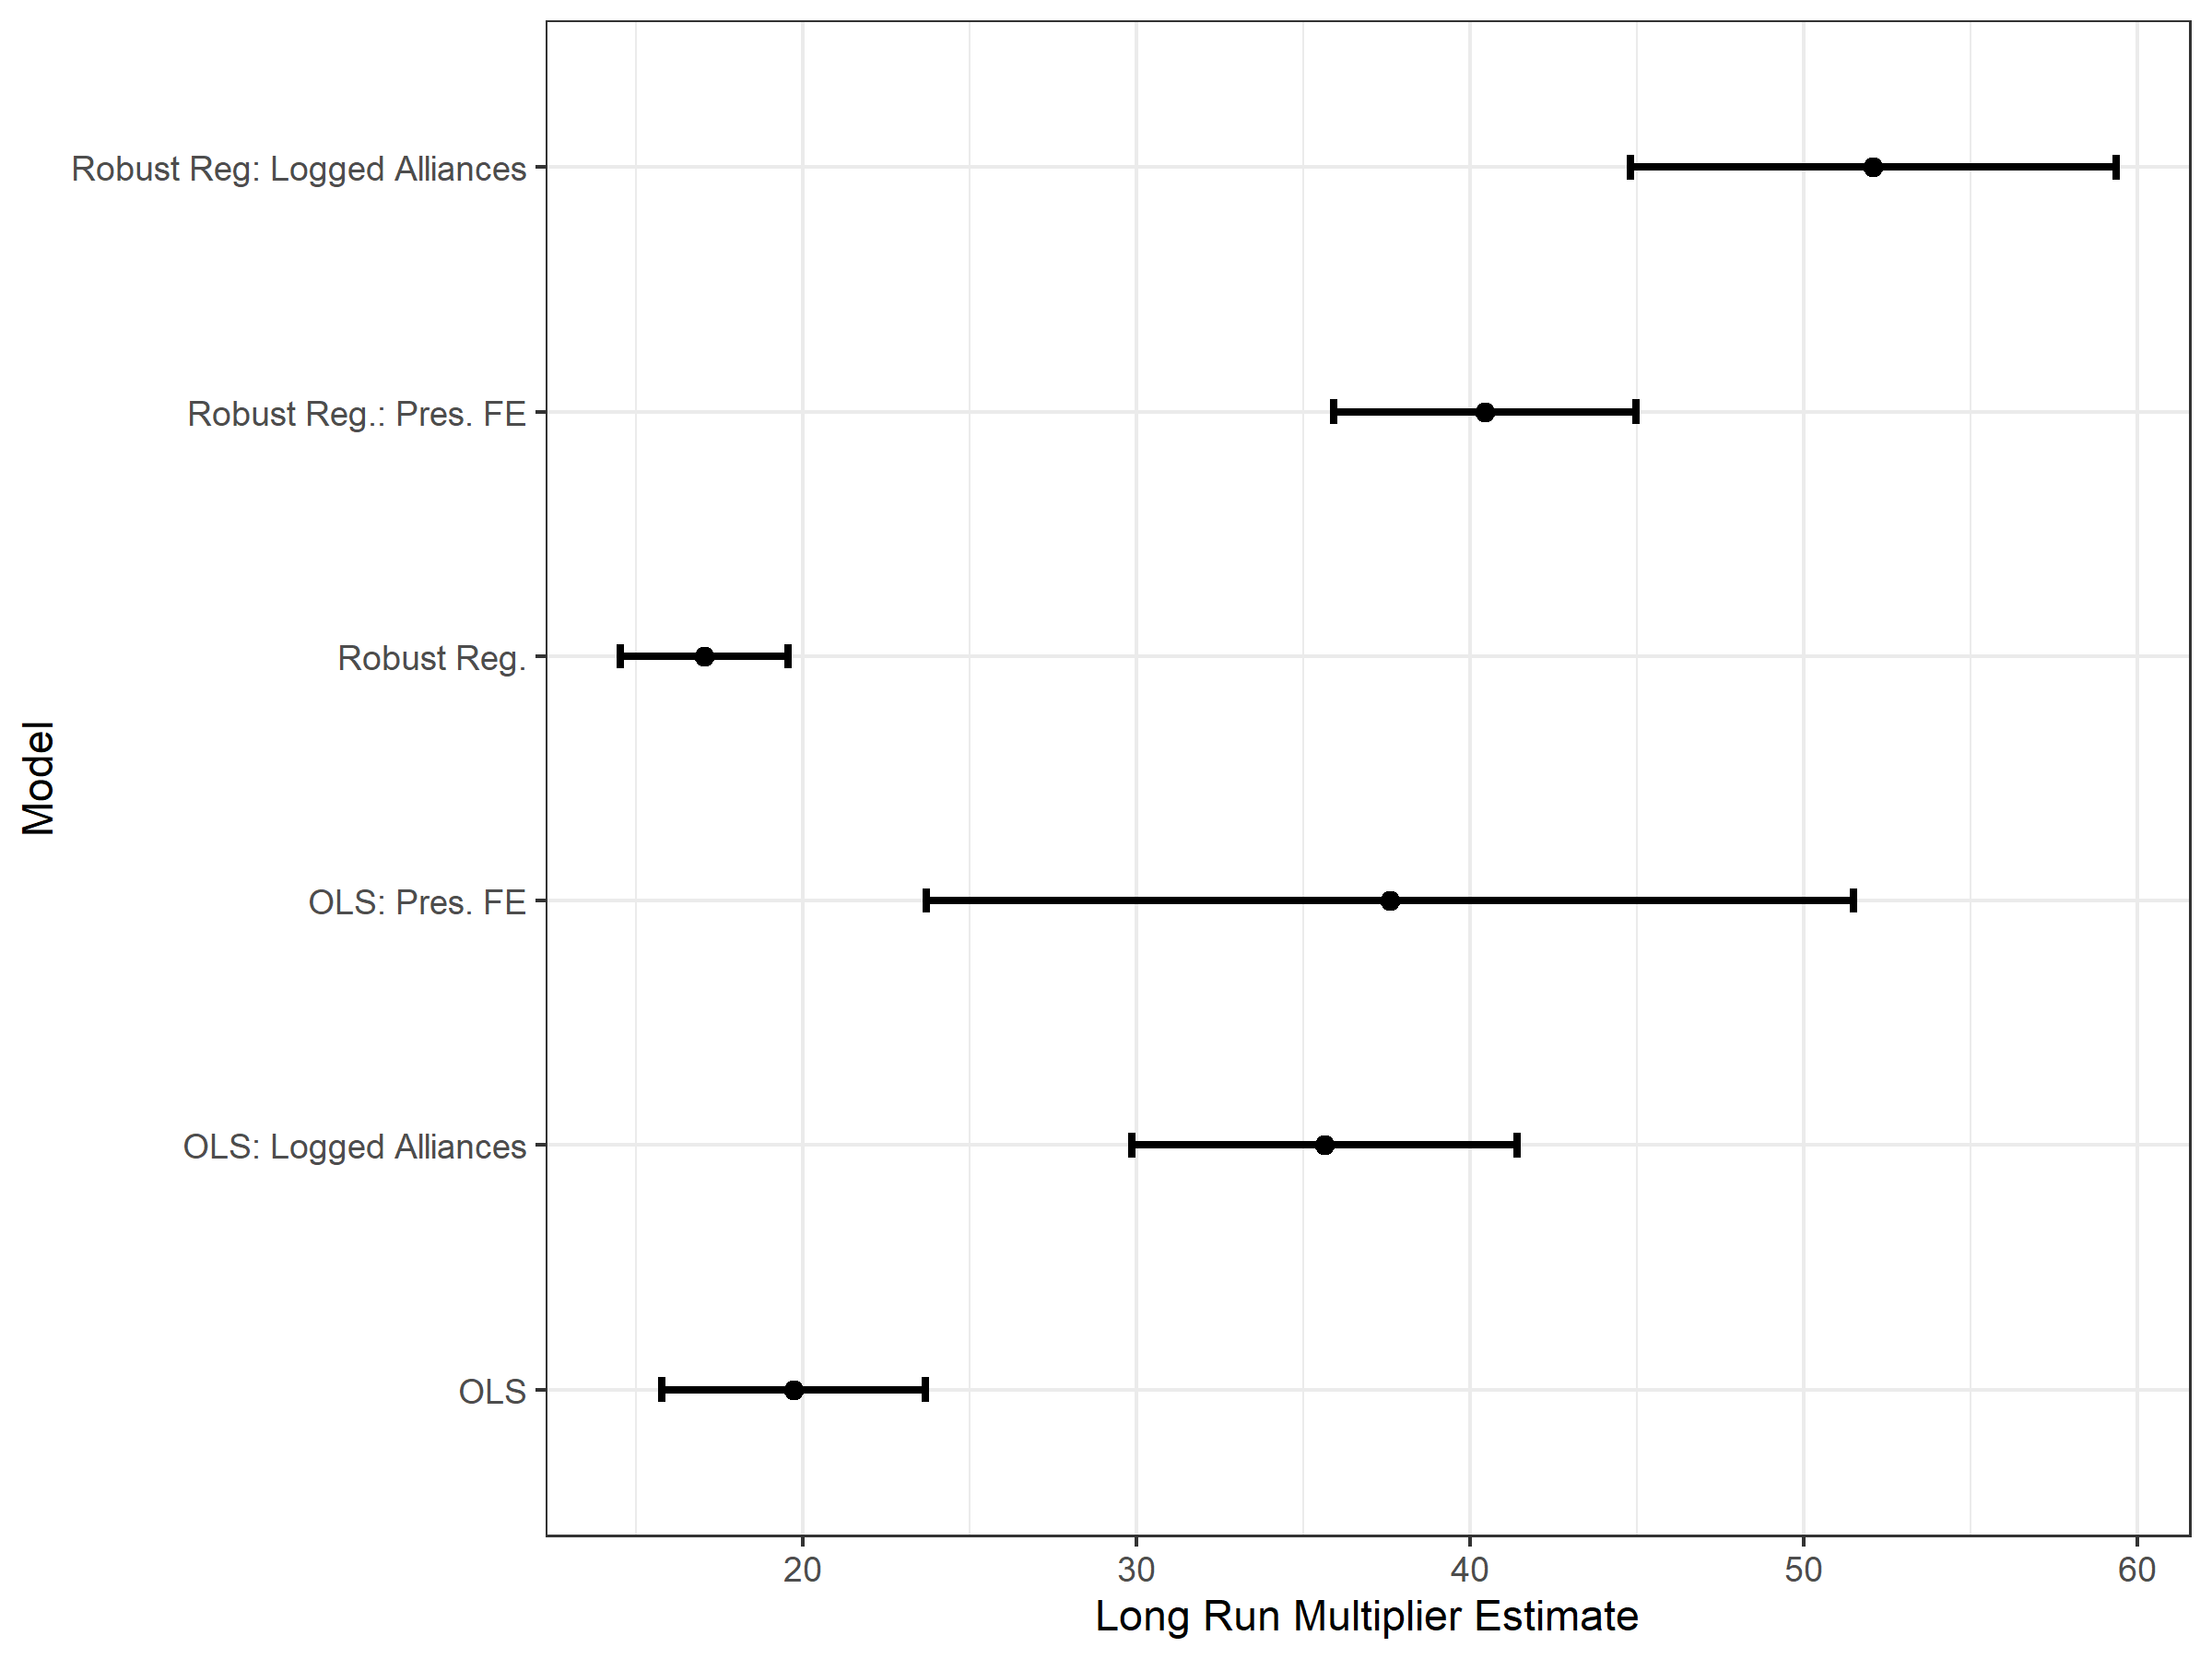
\includegraphics[width = .95\textwidth]{lrm-rob-pre45.png}
\caption{U.S. alliance commitments and military spending from 1920 to 2019.}
\label{fig:lrm-rob-pre45}
\end{figure}


\section{Alternative Lag Structures}

The models in the paper use one lag of alliance commitments and one lag of military spending to model the level of military spending. 
We selected this lag structure using a mix of theoretical and empirical considerations. 
For example, as we note in the manuscript, we lagged the alliance variable because theory suggests that new alliances are unlikely to immediately drive up defense spending. 


Although we do not reject the null hypothesis at conventional levels, alternative lag structures might affect our inferences. 
In this section, we consider two alternative models. 
The first model includes two lags of military spending, making it an ADL(2, 1) model.
Given uncertainty about the dynamic properties of our outcome, this adjustment may not be appropriate \citep{CookWebb2021}.
We also consider a model that includes alliance commitments in current levels and lags. 


\autoref{tab:adl-coefs-lags} presents the key coefficient estimates from these two models. 
The second lag of military spending is negative, which implies a potential reversion in the long run. 
In the model with alliance commitments in lags and levels, the level of alliance commitments has much greater magnitude. 


\begin{table}[!htbp] \centering 
\begin{tabular}{@{\extracolsep{5pt}}lcc} 
\\[-1.8ex]\hline \\[-1.8ex] 
\\[-1.8ex] & \multicolumn{2}{c}{Military Spending} \\ 
\\[-1.8ex] & (1) & (2)\\ 
\hline \\[-1.8ex] 
 Lagged Military Spending & 0.819$^{}$ & 0.419$^{}$ \\ 
  & (0.585, 1.053) & (0.286, 0.552) \\ 
  Second Lag Military Spend. & $-$0.284$^{}$ &  \\ 
  & ($-$0.416, $-$0.153) &  \\ 
  Lag Alliance Commitments & 4.284$^{}$ & 2.439 \\ 
  & (0.716, 7.851) & ($-$3.611, 8.489) \\ 
  Alliance Commitments &  & 8.035$^{}$ \\ 
  &  & (2.047, 14.023) \\ 
  Lag Change in GDP & $-$0.016 & $-$0.067$^{}$ \\ 
  & ($-$0.080, 0.048) & ($-$0.132, $-$0.002) \\ 
  Cold War & $-$7.266 & $-$6.661 \\ 
  & ($-$30.931, 16.399) & ($-$32.206, 18.884) \\ 
  Post-Conflict Years & 6.239$^{}$ & 8.409$^{}$ \\ 
  & (2.542, 9.936) & (4.641, 12.177) \\ 
  Log Combat Fatalities & 18.281$^{}$ & 16.475 \\ 
  & ($-$2.850, 39.413) & ($-$6.370, 39.319) \\ 
  Lag Republican President & $-$2.131 & $-$0.043 \\ 
  & ($-$8.262, 4.000) & ($-$6.596, 6.510) \\ 
  Lag Budget Deficit & 0.060 & 0.017 \\ 
  & ($-$0.032, 0.152) & ($-$0.080, 0.115) \\ 
  Lag Major Power Rival Spending & $-$26.415 & 41.968 \\ 
  & ($-$97.339, 44.510) & ($-$30.876, 114.813) \\ 
  Constant & 6.555 & $-$267.133$^{}$ \\ 
  & ($-$157.382, 170.492) & ($-$417.577, $-$116.689) \\ 
 N & 73 & 73 \\ 
\hline \\[-1.8ex] 
\multicolumn{3}{l}{95\% Confidence Intervals in Parentheses.} \\ 
\end{tabular} 
  \caption{Alternative specifications of the dynamic relationship between U.S. alliance commitments and military spending, 1947-2019. Model one is an ADL(2,1) model with one lag of alliance commitments and two lags of military spending. Model two adds the level of alliance commitments.} 
  \label{tab:adl-coefs-lags} 
\end{table} 


These two specifications give very similar inferences about the long-run relationship between alliance commitments and military spending. 
In general, the LRM is the sum of the alliance coefficients divided by one minus the lagged dependent variable coefficients \citep{CookWebb2021}.
The ADL(2,1) model with two lags of military spending and lagged alliance commitments estimates that the long-run impact of a new alliance commitment is between \$6.5 and 15.7 billion. 
This is the more conservative estimate that we reference in the manuscript. 
A model with lagged and current levels of alliance commitments has an estimated long-run multiplier between \$12 and 20 billion, which is very similar to the estimates in the manuscript. 
Again, this implies that after the US makes a new alliance commitment, the defense budget is between \$12 and 20 billion greater after a few years, and remains as such unless alliance commitments fall or other factors shift defense spending.


\section{List of Current U.S. Allies}

Finally, \autoref{tab:us-ally-list} lists current U.S. allies, along with the year when the United States made a formal defensive alliance commitment for treaties from 1946 on.

\begin{longtable}[!htbp]{| c | c | c |} 
\caption{List of states with a defensive alliance with the United States in 2020. \label{tab:us-ally-list}} \\ 
  \hline
 & Country & Year of Initial Commitment \\ 
  \hline
1 & Haiti & 1946 \\ 
  2 & Dominican Republic & 1946 \\ 
  3 & Mexico & 1946 \\ 
  4 & Guatemala & 1946 \\ 
  5 & Honduras & 1946 \\ 
  6 & El Salvador & 1946 \\ 
  7 & Nicaragua & 1946 \\ 
  8 & Costa Rica & 1946 \\ 
  9 & Panama & 1946 \\ 
  10 & Colombia & 1946 \\ 
  11 & Venezuela & 1946 \\ 
  12 & Ecuador & 1946 \\ 
  13 & Peru & 1946 \\ 
  14 & Brazil & 1946 \\ 
  15 & Bolivia & 1946 \\ 
  16 & Paraguay & 1946 \\ 
  17 & Chile & 1946 \\ 
  18 & Argentina & 1946 \\ 
  19 & Uruguay & 1946 \\ 
  20 & Portugal & 1946 \\ 
  21 & Canada & 1949 \\ 
  22 & United Kingdom & 1949 \\ 
  23 & Netherlands & 1949 \\ 
  24 & Belgium & 1949 \\ 
  25 & Luxembourg & 1949 \\ 
  26 & France & 1949 \\ 
  27 & Italy & 1949 \\ 
  28 & Norway & 1949 \\ 
  29 & Denmark & 1949 \\ 
  30 & Iceland & 1949 \\ 
  31 & Greece & 1951 \\ 
  32 & Turkey & 1951 \\ 
  33 & Japan & 1951 \\ 
  34 & Philippines & 1951 \\ 
  35 & Australia & 1951 \\ 
  36 & South Korea & 1953 \\ 
  37 & Pakistan & 1954 \\ 
  38 & Thailand & 1954 \\ 
  39 & Spain & 1963 \\ 
  40 & Trinidad \& Tobago & 1967 \\ 
  41 & Barbados & 1967 \\ 
  42 & Jamaica & 1969 \\ 
  43 & Grenada & 1975 \\ 
  44 & Suriname & 1977 \\ 
  45 & Dominica & 1979 \\ 
  46 & St. Lucia & 1979 \\ 
  47 & St. Vincent \& Grenadines & 1981 \\ 
  48 & Antigua \& Barbuda & 1981 \\ 
  49 & Bahamas & 1982 \\ 
  50 & St. Kitts \& Nevis & 1984 \\ 
  51 & Germany & 1990 \\ 
  52 & Belize & 1991 \\ 
  53 & Guyana & 1991 \\ 
  54 & Poland & 1997 \\ 
  55 & Hungary & 1997 \\ 
  56 & Czechia & 1997 \\ 
  57 & Slovakia & 2003 \\ 
  58 & Slovenia & 2003 \\ 
  59 & Bulgaria & 2003 \\ 
  60 & Romania & 2003 \\ 
  61 & Estonia & 2003 \\ 
  62 & Latvia & 2003 \\ 
  63 & Lithuania & 2003 \\ 
  64 & Albania & 2008 \\ 
  65 & Croatia & 2008 \\ 
  66 & Montenegro & 2016 \\ 
  67 & North Macedonia & 2020 \\ 
   \hline
\end{longtable}


In addition to the list of current U.S. allies, \autoref{tab:us-oldally-list} lists countries that had a U.S. alliance at some time after 1945, but no longer have an alliance treaty with the United States. 
Israel and Taiwan are both U.S. partners, but neither has a formal alliance commitment. 

\begin{table}[ht]
\centering
\begin{tabular}{rlrr}
  \hline
 & Country & Alliance Treaty Start & Alliance Treaty End \\ 
  \hline
1 & Cuba & 1946 & 1962 \\ 
  2 & Iran & 1959 & 1979 \\ 
  3 & Israel & 1981 & 1991 \\ 
  4 & Taiwan & 1954 & 1980 \\ 
  5 & New Zealand & 1951 & 1986 \\ 
   \hline
\end{tabular}
\caption{List of past formal U.S. treaty allies.} 
\label{tab:us-oldally-list}
\end{table}



\newpage
\singlespace

\bibliography{../us-all-milex-bib}


\end{document}




